%%
%% Copyright 2007, 2008, 2009 Elsevier Ltd
%%
%% This file is part of the 'Elsarticle Bundle'.
%% ---------------------------------------------
%%
%% It may be distributed under the conditions of the LaTeX Project Public
%% License, either version 1.2 of this license or (at your option) any
%% later version.  The latest version of this license is in
%%    http://www.latex-project.org/lppl.txt
%% and version 1.2 or later is part of all distributions of LaTeX
%% version 1999/12/01 or later.
%%
%% The list of all files belonging to the 'Elsarticle Bundle' is
%% given in the file `manifest.txt'.
%%

%% Template article for Elsevier's document class `elsarticle'
%% with numbered style bibliographic references
%% SP 2008/03/01
%%
%%
%%
%% $Id: elsarticle-template-num.tex 4 2009-10-24 08:22:58Z rishi $
%%
%%
\documentclass[preprint,12pt]{elsarticle}

%% Use the option review to obtain double line spacing
%% \documentclass[preprint,review,12pt]{elsarticle}

%% Use the options 1p,twocolumn; 3p; 3p,twocolumn; 5p; or 5p,twocolumn
%% for a journal layout:
%% \documentclass[final,1p,times]{elsarticle}
%% \documentclass[final,1p,times,twocolumn]{elsarticle}
%% \documentclass[final,3p,times]{elsarticle}
%% \documentclass[final,3p,times,twocolumn]{elsarticle}
%% \documentclass[final,5p,times]{elsarticle}
%% \documentclass[final,5p,times,twocolumn]{elsarticle}





\newcommand{\hpl}{Hephaestus-PL}
\newcommand{\hp}{Hephaestus}


%% if you use PostScript figures in your article
%% use the graphics package for simple commands
%% \usepackage{graphics}
%% or use the graphicx package for more complicated commands
%% \usepackage{graphicx}
%% or use the epsfig package if you prefer to use the old commands
%% \usepackage{epsfig}

%% The amssymb package provides various useful mathematical symbols
\usepackage{amssymb}

\usepackage{multirow}

%% The amsthm package provides extended theorem environments
%% \usepackage{amsthm}

%% The lineno packages adds line numbers. Start line numbering with
%% \begin{linenumbers}, end it with \end{linenumbers}. Or switch it on
%% for the whole article with \linenumbers after \end{frontmatter}.
%% \usepackage{lineno}

%% natbib.sty is loaded by default. However, natbib options can be
%% provided with \biboptions{...} command. Following options are
%% valid:

%%   round  -  round parentheses are used (default)
%%   square -  square brackets are used   [option]
%%   curly  -  curly braces are used      {option}
%%   angle  -  angle brackets are used    <option>
%%   semicolon  -  multiple citations separated by semi-colon
%%   colon  - same as semicolon, an earlier confusion
%%   comma  -  separated by comma
%%   numbers-  selects numerical citations
%%   super  -  numerical citations as superscripts
%%   sort   -  sorts multiple citations according to order in ref. list
%%   sort&compress   -  like sort, but also compresses numerical citations
%%   compress - compresses without sorting
%%
%% \biboptions{comma,round}

% \biboptions{}

\usepackage[usenames,dvipsnames]{xcolor}
\usepackage{subfigure}

%\usepackage{color}
\usepackage{listings}

\definecolor{gray}{RGB}{220,220,220}
\journal{Science of Computer Programming}

%\lstloadlanguages{Haskell}
%\lstnewenvironment{code}
%    {\lstset{}%
%      \csname lst@SetFirstLabel\endcsname}
%    {\csname lst@SaveFirstLabel\endcsname}
%    \lstset{
%      basicstyle=\small\ttfamily,
%      backgroundcolor=\color{gray},
%      flexiblecolumns=false,
%      basewidth={0.5em,0.45em},
%      literate={+}{{$+$}}1 {/}{{$/$}}1 {*}{{$*$}}1 {=}{{$=$}}1
%               {>}{{$>$}}1 {<}{{$<$}}1 {\\}{{$\lambda$}}1
%               {\\\\}{{\char`\\\char`\\}}1
%               {->}{{$\rightarrow$}}2 {>=}{{$\geq$}}2 {<-}{{$\leftarrow$}}2
%               {<=}{{$\leq$}}2 {=>}{{$\Rightarrow$}}2
%               {\ .}{{$\circ$}}2 {\ .\ }{{$\circ$}}2
%               {>>}{{>>}}2 {>>=}{{>>=}}2
%               {|}{{$\mid$}}1
%    }

\lstdefinelanguage{haskell}{%
%  numbers=none,
  morekeywords={do,module,qualified,import,let,case,of,in,class,instance,data,newtype,where,otherwise,deriving,type,extends,public,forall},
  sensitive=true,
  morecomment=[l]{--},
  morecomment=[s]{/*}{*/},
  morestring=[b]",
}

\lstset{%
  frame=none,
  xleftmargin=2pt,
  stepnumber=1,
  numbers=left,
  numbersep=5pt,
  numberstyle=\ttfamily\tiny\color[gray]{0.3},
  belowcaptionskip=\bigskipamount,
  captionpos=b,
  escapeinside={*'}{'*},
  language=haskell,
  tabsize=2,
  emphstyle={\bf},
  commentstyle=\it,
  stringstyle=\mdseries\rmfamily,
  showspaces=false,
  keywordstyle=\bfseries\rmfamily,
  columns=flexible,
  basicstyle=\small\sffamily,
  showstringspaces=false,
  morecomment=[l]\%,
}


\begin{document}

\begin{frontmatter}

%% Title, authors and addresses

%% use the tnoteref command within \title for footnotes;
%% use the tnotetext command for the associated footnote;
%% use the fnref command within \author or \address for footnotes;
%% use the fntext command for the associated footnote;
%% use the corref command within \author for corresponding author footnotes;
%% use the cortext command for the associated footnote;
%% use the ead command for the email address,
%% and the form \ead[url] for the home page:
%%
%% \title{Title\tnoteref{label1}}
%% \tnotetext[label1]{}
%% \author{Name\corref{cor1}\fnref{label2}}
%% \ead{email address}
%% \ead[url]{home page}
%% \fntext[label2]{}
%% \cortext[cor1]{}
%% \address{Address\fnref{label3}}
%% \fntext[label3]{}

\title{Supporting Configurability and Flexibility in Software Product Line Tool Development: the \hpl{} Case}
%\title{On the Design and Implementation of \hpl: a Software Product Line of Software Product Line Tools}

%% use optional labels to link authors explicitly to addresses:
%% \author[label1,label2]{<author name>}
%% \address[label1]{<address>}
%% \address[label2]{<address>}

\author[unb]{Lucin\'{e}ia Turnes}
\ead{lucineiaturnes@gmail.com}
\author[ukob]{Ralf L\"{a}mmel}
\ead{rlaemmel@gmail.com}
\author[unb]{Vander Alves\corref{cor1}}
\author[unb]{Rodrigo Bonif\'{a}cio}
\ead{rbonifacio@cic.unb.br}
\cortext[cor1]{Corresponding author. Telephone: +55 61 8157-1464. Fax: +55 61 3107-7414.}
\ead{valves@unb.br}

\address[unb]{Departamento de Ci\^{e}ncia da Computa\c{c}\~{a}o, Universidade de Bras\'{i}lia, Campus Darcy Ribeiro, Bras\'{i}lia, Brazil, 70910-900}
\address[ukob]{Software Languages Team, Universit\"{a}t Koblenz-Landau, Institut f\"{u}r Informatik, Universittsstrae 1, D-56070 Koblenz, Germany}




\author{}

\address{}

\begin{abstract}
%context
Tool support is essential for application engineering in software product lines.
%problem
Despite a myriad of existing tools, most still lack adequate support for configurability and flexibility, so that it is hard for them to be applied in different contexts, e.g., addressing variability in an arbitrary combination of different artifacts and introducing and managing variability in new artifacts.
% solution
Addressing this issue requires systematically exploring underlying commonality and adequately managing variability of such tools. Accordingly, this paper presents domain analysis, design, implementation, and a supporting process for extending \hpl, a software product line of software product line tools. Hephaestus-PL is supported by a process allowing instantiating product line tools for modeling variability in new and in any combination of artifacts, and has been developed by bootstrapping previous versions of the Hephaestus tool.
%Evidence
An assessment reveals that it has improved configurability and flexibility when compared to previous evolution of Hephaestus.

\end{abstract}

\begin{keyword}
%% keywords here, in the form: keyword \sep keyword
Software Product Line Tools \sep Multi-artifact variability management \sep  Bootstrapping

%% MSC codes here, in the form: \MSC code \sep code
%% or \MSC[2008] code \sep code (2000 is the default)

\end{keyword}

\end{frontmatter}

%%
%% Start line numbering here if you want
%%
% \linenumbers

%%%%%%%%%%%%%%%%%%%%%%%%%%%%%%%%%%%%%%%%%%%%%%%%%%

\section{Introduction}
\label{introduction}

%%%%%%%%%%%%%%%%%%%%%%%%%%%%%%%%%%%%%%%%%%%%%%%%%%

% Context: SPL derivation tools

A Software Product Line (SPL) is a set of software-intensive systems that share a common, managed set of features satisfying the specific needs of a particular market segment or mission and that are developed from a common set of core assets in a prescribed way~\cite{spl-book}. Potential benefits include improved productivity with lower development costs and time-to-market and increased quality. To achieve these benefits, tool support for the underlying activities is essential. In particular, this holds for Application Engineering, in which a product is defined by selecting a group of features and then parts of different components are combined. Given the inherent complexity of SPLs and the coordination required for instantiation, the process of derivation of individual products from shared software assets should be supported by tools: \emph{product derivation tools}. Without such tools, the derivation process is a laborious, error-prone, and thus, expensive activity~\cite{griss,deelstra:2005}.

%%%%%%%%%%%%%%%%%%%%%%%%%%%%%%%%%%%%%%%%%%%%%%%%%%

% Problem:

The changing needs of users and the continuous evolution of product lines motivates configurability and extensibility of product derivation tools for addressing future needs. As reported by a contemporary Systematic Literature Review and expert survey~\cite{ist-2010}, key requirements of product derivation tools are indeed configurability and extensibility (in fact, `flexibility' in the terminology of~\cite{ist-2010}) which the same study identifies as shortcoming of most existing tools. The present paper addresses such configurability and extensibility. As an illustration of insufficient configurability, consider a derivation tool that targets different types of artifacts without supporting, though, the selection of types for a specific use case of the tool. For instance, different variants of the Haskell-based \hp{} tool~\cite{rbonifacio:sbcars2009} for product derivation target use case models, requirement models, source code, and yet other types of artifacts, but the selection of only some of the types is not possible for a given variant of \hp. The present paper studies \hp{} in detail and improves it ultimately. As an illustration of insufficient extensibility, consider a derivation tool that needs to target an additional type of artifact without providing, though, any extension scheme and process to this end. For instance, \hp{} had to target architectural models at some point, but this extension could only be completed in a low-level (i.e., laborious and error-prone) manner.

%%%%%%%%%%%%%%%%%%%%%%%%%%%%%%%%%%%%%%%%%%%%%%%%%%

% Challenge

The requested configurability and extensibility may be obtainable, if the variability within tools for product derivation is managed by architecting the tools themselves as SPLs, as suggested by Gr{\"u}nbacher et al.~\cite{grunbacher:2008} and also exemplified by some efforts~\cite{grunbacher:2011,batory-ahead-bootstrap}. Overall, the major contribution of the present paper is the description of the details of the engineering process for obtaining and enhancing such a meta-product line, while using the Haskell-based \hp{} tool for product derivation for a comprehensive study.

%%%%%%%%%%%%%%%%%%%%%%%%%%%%%%%%%%%%%%%%%%%%%%%%%%

\subsection*{Contributions of the Paper}

\begin{itemize}

\item We describe an extractive process that enhances the existing Haskell-based tool \hp{} for deriving products from a SPL into a Haskell-based proper product line, \hpl, for product derivation tools. In particular, we describe domain analysis, design, and implementation~\cite{gpbook} of \hpl. Configuration is expressive; specifically, or-features (allowing for combinations) are supported as opposed to just alternative features (allowing only for exclusive choices). \hpl{} employes a general transformational approach to variable management. In this manner, the present paper provides evidence for the feasibility of configurable and extensible tools for product derivation.

\item We describe the technicalities and implications of providing a meta-SPL in Haskell. \hpl's transformational approach is implemented through metaprogramming in Haskell. Technically, we had to solve an \hp-specific variation on the `Expression Problem'~\cite{Wadler98,Lopez-HerrejonBC05} within Haskell. The approach enables modular code organization for all components of \hpl, separate compilation within limits, and bootstrapping of \hpl, thereby achieving high uniformity across the regular SPL level and the meta-SPL level.

\item We describe a reactive process for evolving \hpl{} for modeling variability for new types of artifacts so that product line tools can be derived for these new types. An assessment reveals that \hpl{} has improved configurability and extensibility when compared to previous variants of \hp. In this manner, the present paper provides evidence for the effectiveness of addressing the problem of configurable and extensible tools for product derivation.

\end{itemize}

We believe that these contributions and experiences could be leveraged in other contexts in which configurability and extensibility of tools for product derivation are key requirements. 

%%%%%%%%%%%%%%%%%%%%%%%%%%%%%%%%%%%%%%%%%%%%%%%%%%

\subsection*{Road-map of the Paper}

The remainder of this paper is organized as follows. First, Section~\ref{sec:hephaestus} briefly describes \hp{} and it analyzes a representative evolution scenario for addressing an additional type of artifacts. Next, based on experience with variants and evolution history of \hp, Section~\ref{sec:domainAnalysis}--\ref{sec:implementation} describe 
domain analysis, domain design, and implementation of \hpl. Section~\ref{sec:process} describes a reactive process for extending \hpl. Section~\ref{sec:results-discussion} provides an assessment and discussion of \hpl. Related work is addressed in Section~\ref{related-work}. The paper is concluded in Section~\ref{conclusion}. 

The Haskell source code of \hpl{} is publically available.\footnote{\url{https://gitorious.org/hephaestus-pl/hephaestus-pl}} For the rest of the paper, `Haskell' refers to standardized Haskell in sense of Haskell 2012\footnote{\url{http://www.haskell.org/onlinereport/haskell2010/}}, unless noted otherwise.

%%%%%%%%%%%%%%%%%%%%%%%%%%%%%%%%%%%%%%%%%%%%%%%%%%


%%%%%%%%%%%%%%%%%%%%%%%%%%%%%%%%%%%%%%%%%%%%%%%%%%

\section{\hp}
\label{sec:hephaestus}

\hp~\cite{rbonifacio:sbcars2009} is a publicly
available\footnote{\url{https://gitorious.org/hephaestus/pages/Home}}
product derivation tool~\cite{deelstra:2005}, which receives
contributions from different institutions (Federal University of
Pernambuco, University of S\~{a}o Paulo, University of
Bras\'{i}lia). Initially developed as a proof-of-concept tool for
managing variabilities in use case
scenarios~\cite{rbonifacio:aosd2009}, \hp{} provides a Haskell-based,
declarative and executable specification of a
compositional~\cite{kastner:2008} and parametric approach for managing
variability in a different asset types.  Currently, \hp{} supports
variability, for example, for use case scenarios, business processes,
Simulink models, and source code; and it has been used as the
derivation tool in a industrial-strength product
line~\cite{ferreira:2010}.

%%%%%%%%%%%%%%%%%%%%%%%%%%%%%%%%%%%%%%%%%%%%%%%%%%

\subsection{Initial \hp}
\label{sec:initial-hp}

For the initial purpose of the tool, the implementation contained the
following entities:

\begin{itemize}
\item Specific data types representing use case models (UCM), feature
  models (FM), and configuration knowledge (CK) model~\cite{gpbook},
  which relates feature expressions in propositional logic to
  transformations that deal with variability in use cases.

\item Specific functions that solve SPL variabilities in use case
  scenarios, by selecting use cases or scenarios from an SPL model,
  composing them, and binding parameters according to specific feature
  configurations.

\item A \texttt{build} function that serves as an interpreter for the
  configuration knowledge and is responsible for building a specific
  product from a given selection of features, i.e., a feature
  configuration (FC).

\item Specific functions providing functionality on use case models.

\end{itemize}

%%%%%%%%%%%%%%%%%%%%%%%%%%%%%%%%%%%%%%%%%%%%%%%%%%

\begin{figure}[t!]
\bigskip
\begin{lstlisting}
type ConfigurationKnowledge = [ConfigurationItem] *'\label{ck-i-1}'*
data ConfigurationItem = ConfigurationItem {
  expression = FeatureExpression,
  transformations = [Transformation]
} *'\label{ck-f-1}'*

build :: FeatureModel *'\label{build-i-1}'*
      -> FeatureConfiguration
      -> ConfigurationKnowledge
      -> SPLModel
      -> InstanceModel
build fm fc ck spl = derive ts spl emptyInstance
where
    ts = concat [transformations c | c <- ck, eval fc (expression c)]
    ucmodel       = splUCM spl
    emptyUCM      = ucmodel { useCases = [] , aspects = [] }
    emptyInstance = InstanceModel fc emptyUCM *'\label{build-f-1}'*

derive [] spl product = product
derive (t:ts) spl product = derive ts spl (t spl product)

type Transformation = SPLModel -> InstanceModel -> InstanceModel *'\label{transf-1}'*

data SPLModel = SPLModel { *'\label{splmodel-i-1}'*
   splFeatureModel :: FeatureModel,
   splUCM :: UseCaseModel
} *'\label{splmodel-f-1}'*

data InstanceModel = InstanceModel { *'\label{instancemodel-i-1}'*
   featureConfiguration :: FeatureConfiguration,
   ucm :: UseCaseModel
} *'\label{instancemodel-f-1}'*

exportProduct :: Path -> InstanceModel -> IO () *'\label{exportP-i-1}'*
exportProduct t product = do
  exportUcmToLatex (t ++ ``/doc.tex'') (ucm product) *'\label{exportP-f-1}'*

exportUcmToLatex = ... -- functionality specific to use case models
\end{lstlisting}
\caption{Code snippet of the initial implementation of \hp.}
\label{fig:hp-initial}
\bigskip
\end{figure}

%%%%%%%%%%%%%%%%%%%%%%%%%%%%%%%%%%%%%%%%%%%%%%%%%%

Figure~\ref{fig:hp-initial} presents a code snippet of
the initial implementation of \hp{} including data types related to
configuration knowledge (lines \ref{ck-i-1}-\ref{ck-f-1}) and the
corresponding interpreter (the \texttt{build} function, in lines
\ref{build-i-1}-\ref{build-f-1}), and the signature of the
transformation functions (line \ref{transf-1}). The configuration
knowledge relates the problem space (through a feature expression) to
the solution space (through a list of asset transformations). Each
transformation solves some variation point in the SPL asset base. The
\texttt{build} function has four input artifacts (FM, FC, CK, and SPL)
and generates a product, i.e., an instance of the SPL. The build
process evaluates the rows of the CK, validating each feature
expression according to the FC--- the set of features that
characterizes a given product. If a feature expression of the CK is
true for the given FC, then the corresponding transformations are
applied to the emerging instance. In addition, the code snippet also
shows the initial representation of the data types \texttt{SPLModel}
(lines \ref{splmodel-i-1}-\ref{splmodel-f-1}) and
\texttt{InstanceModel} (lines
\ref{instancemodel-i-1}-\ref{instancemodel-f-1}). Both types collect
assets and group them with the feature model or the feature
configuration, respectively. The build process eliminates all
variability from the \texttt{SPLModel} value and computes the
\texttt{InstanceModel} value. The \texttt{exportProduct} function
(lines \ref{exportP-i-1}-\ref{exportP-f-1}) generates a \LaTeX\
representation of a product-specific use case model.

%%%%%%%%%%%%%%%%%%%%%%%%%%%%%%%%%%%%%%%%%%%%%%%%%%

\subsection{Evolution of \hp} 
\label{sec:hp-evolution}

In the context of a R\&D project, \hp{} was used as a replacement for
a proprietary tool that was used to manage variabilities in an
industrial-strength product line~\cite{ferreira:2010}. In this
context, \hp{} had to be evolved so that it could manage variability
not only in use case scenarios, but also in higher level requirements
and source code. Variability in source code means here that source
files can be selected for inclusion into the product, triggering
compilation and preprocessing, thereby solve yet more variability
within the source code. We show the configurations for both the
initial release and the evolved releases in
Figure~\ref{fig:hephaestus-conf1a} and
Figure~\ref{fig:hephaestus-conf1b}.

%%%%%%%%%%%%%%%%%%%%%%%%%%%%%%%%%%%%%%%%%%%%%%%%%%

\begin{figure*}[t!]
\begin{center}
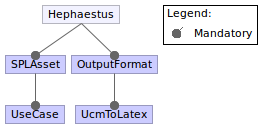
\includegraphics[scale=0.6]{imagens/conf1a-hp.png}
\caption{Configuration of \hp{} in the first release.}
\label{fig:hephaestus-conf1a}
\end{center}
\end{figure*}

%%%%%%%%%%%%%%%%%%%%%%%%%%%%%%%%%%%%%%%%%%%%%%%%%%

\begin{figure*}[t!]
\begin{center}
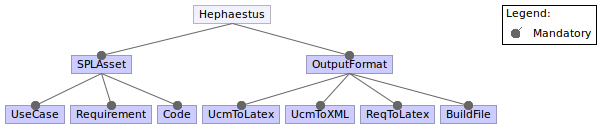
\includegraphics[scale=0.6]{imagens/conf1b-hp.png}
\caption{Configuration of \hp{} in the second release.}
\label{fig:hephaestus-conf1b}
\end{center}
\end{figure*}

%%%%%%%%%%%%%%%%%%%%%%%%%%%%%%%%%%%%%%%%%%%%%%%%%%

Evolution required that new data types and transformations were added
and some of the existing code had to be changed. Precisely, to
introduce support for variability in high-level requirements (or
requirements for short) and source code, the following implementation
and evolution steps were necessary:

\begin{enumerate}[(a)]

\item Implementation of new data types for representing requirements
  and references to source-code assets.

\item Implementation of new parsing and output functions for
  reading/writing requirements and source-code assets into/from \hp.

\item Implementation of new transformations for resolving
  variabilities in requirements and source code.

\item Evolution of the configuration knowledge XML parser so that it
  could recognize the concrete syntax of the new transformations.

\item Evolution of the base product instance used by the \texttt{build}
  function.

\item Evolution of both, \texttt{SPLModel} and \texttt{InstanceModel}
  data types, to collect new assets.

\end{enumerate}

%%%%%%%%%%%%%%%%%%%%%%%%%%%%%%%%%%%%%%%%%%%%%%%%%%

\begin{figure}[t!]
\bigskip
\begin{lstlisting}
data SPLModel = SPLModel { *'\label{splmodel-i-2}'*
   splFeatureModel :: FeatureModel,
   splUCM :: UseCaseModel,
   splReq :: RequirementModel,
   splComponents :: ComponentModel *'\label{splComponents-2}'*
} *'\label{splmodel-f-2}'*

data InstanceModel = InstanceModel { *'\label{instancemodel-i-2}'*
   featureConfiguration :: FeatureConfiguration,
   ucm :: UseCaseModel,
   req :: RequirementModel,
   components :: ComponentModel, *'\label{components-2}'*
   buildEntries :: [PreprocessingDirective], *'\label{buildEntries-2}'*
   preProcessFiles :: [PreprocessingFiles] *'\label{preProcessFiles-2}'*
} *'\label{instancemodel-f-2}'*

build :: FeatureModel -> FeatureConfiguration 
      -> ConfigurationKnowledge -> SPLModel -> InstanceModel
build fm fc ck spl = derive ts spl emptyInstance
where
    ts = concat [transformations c | c <- ck, eval fc (expression c)]
    ucmodel       = splUCM spl
    emptyUCM      = ucmodel { useCases = [] , aspects = [] }  *'\label{emptyInstance-i-2}'*
    emptyReq      = RM { reqs = [] }
    emptyInstance = InstanceModel fc emptyUCM emptyReq [] [] [] *'\label{emptyInstance-f-2}'*

exportProduct :: FilePath -> FilePath -> InstanceModel -> IO ()  *'\label{exportP-i-2}'*
exportProduct s o product = do
  exportUcmToLatex (o ++ ``/doc.tex'') (ucm product)
  exportRequirementsToLatex (o ++ ``/doc.lst'') (req product)
  exportSourceCode s o product  *'\label{exportP-f-2}'*

exportRequirementsToLatex :: FilePath -> RequirementModel -> IO ()
exportSourceCode o rm = ... -- functionality dealing with source code

exportSourceCode :: FilePath -> FilePath -> InstanceModel -> IO ()
exportSourceCode s o p = ... -- functionality dealing with source code
\end{lstlisting}
\caption{\texttt{SPLModel} and \texttt{InstanceModel} data types,
  \texttt{emptyInstance} definition and \texttt{exportProduct}
  function after introducing support for managing variabilities in
  requirements and source code.}
\label{fig:spl-model-with-req-and-code}
\bigskip
\end{figure}

%%%%%%%%%%%%%%%%%%%%%%%%%%%%%%%%%%%%%%%%%%%%%%%%%%

The evolution of data types and functions of \hp{}, as described
above, is illustrated in Figure~\ref{fig:spl-model-with-req-and-code}
and Figure~\ref{fig:xml-transformation-parser}. To introduce support
for new types of artifacts, we have to change the \texttt{SPLModel}
data type (lines \ref{splmodel-i-2}-\ref{splmodel-f-2} in
Figure~\ref{fig:spl-model-with-req-and-code}), the
\texttt{InstanceModel} data type (lines
\ref{instancemodel-i-2}-\ref{instancemodel-f-2}), the empty product
definition (lines \ref{emptyInstance-i-2}-\ref{emptyInstance-f-2}),
the \texttt{exportProduct} function (lines
\ref{exportP-i-2}-\ref{exportP-f-2}), and the
\texttt{xml2Transformation} function of the XML parser for
configuration knowledge (Figure~\ref{fig:xml-transformation-parser}).

In contrast, the data types \texttt{ConfigurationKnowledge} and
\texttt{FeatureModel} as well as the \texttt{build} function do not
require any revision, when we introduce variability support for new
types of artifacts.

In particular, evolving \hp{} to support source code variability
(Figure~\ref{fig:spl-model-with-req-and-code}) required a new type of
asset in the \texttt{SPLModel} (\texttt{splComponents}, line
\ref{splComponents-2}). This asset is a list of pairs that relate a
name to the relative path of a source code file. The same type of
asset was also introduced into the \texttt{InstanceModel} (line
\ref{components-2}). Besides that, two other fields were required in
the InstanceModel: (a) \texttt{buildEntries} (line
\ref{buildEntries-2}), which declares pre-processing directives, and
(b) \texttt{preProcessFiles} (line \ref{preProcessFiles-2}), which
declares a list of files that should be pre-processed by a third party
tool. These fields are instantiated when \hp{} builds a product.

%%%%%%%%%%%%%%%%%%%%%%%%%%%%%%%%%%%%%%%%%%%%%%%%%%

\begin{figure}[t!]
\begin{lstlisting}
xml2Transformation :: XmlTransformation -> Parser Transformation
xml2Transformation transformation =
let
  args = ...
  tnsName = xmlTransformationName transformation
in
  case tnsName of
   "selectScenarios" -> Success (selectScenarios args) *'\label{transformations-ucm-i-2}'*
   "selectUseCases" -> Success (selectUseCases args)
   "evaluateAspects" -> Success (evaluateAspects args)
   "bindParameter" -> ...  *'\label{transformations-ucm-f-2}'*
   "selectRequirements" -> ... *'\label{transformations-req-2}'*
   "selectComponents" -> ... *'\label{transformations-code-i-2}'*
   "selectAndMoveComponent" -> ...
   "createBuildEntries" -> ...
   "preprocessFiles" -> ... *'\label{transformations-code-f-2}'*
   _ -> Fail ``...''
\end{lstlisting}
\caption{Code snippet for the XML parser for configuration knowledge}
\label{fig:xml-transformation-parser}
\end{figure}

%%%%%%%%%%%%%%%%%%%%%%%%%%%%%%%%%%%%%%%%%%%%%%%%%%

The code snippet in Figure~\ref{fig:xml-transformation-parser} shows
the revised XML parser for configuration knowledge. The initial
version of \hp{} declared just the first four case statements on the
\texttt{xml2Transformation} function (lines
\ref{transformations-ucm-i-2}-\ref{transformations-ucm-f-2}). The
added \texttt{selectRequirements} transformation (line
\ref{transformations-req-2}) deals with variability in the
requirements models, whereas the remaining transformations (lines
\ref{transformations-code-i-2}-\ref{transformations-code-f-2}) deal
with variability in source code. 

Likewise, \hp{} also provides limited configurability: to obtain a new
version of \hp{} managing variability in only a proper subset of the
types of artifacts currently supported (use cases, requirements,
source code), e.g., a version supporting only source code and use
cases, the change impact is similar to what has been described
previously when extending \hp{} to target new types of artifacts.

%%%%%%%%%%%%%%%%%%%%%%%%%%%%%%%%%%%%%%%%%%%%%%%%%%

\subsection{\hp's `Expression Problem'}
\label{sec:ep}

Technically, the evolution scenario demonstrated an extensibility
problem. We had to extend data types and functions to incorporate new
types of artifacts, transformations, and support functionality (e.g., for
exporting). We failed to provide a modular extension; instead, we
ended up revising existing code.

The well-known `Expression Problem'
(EP~\cite{Wadler98,Lopez-HerrejonBC05}) captures this sort of
challenge in a principle manner: \emph{Given a family of data variants
  and a family of operations on the data, how can we design an
  implementation of data and operations such that new variants and new
  operations can be added without revising existing code, while
  possibly also providing some degree of separate compilation, modular
  type checking, and modular reasoning?}

Programming language support for the EP, as discussed for Haskell as
the underlying language below, helps with modularization so that
evolution scenarios, like the one discussed above, can be potentially
carried out accordingly.

Hinze and L\"oh proposed a Haskell extension for open data types and
functions for Haskell~\cite{LoehH06}, which would provide a solution
to the EP in Haskell. The extension allows adding new cases to data
types (i.e., adding cases to `sums', algebraically speaking) and new
equations to functions (i.e., adding cases to a discrimination over a
sum), but it does not deal with additional adaptation patterns
encountered in
Figure~\ref{fig:spl-model-with-req-and-code}. Specifically, the
evolution of \hp{} involved extending `products' as opposed to just
`sums' (see the data types \texttt{SPLModel} and
\texttt{InstanceModel}) and `function compositions' as opposed to just
`case discriminations' (see the the function \texttt{exportProduct}).
Arguably, these adaptation patterns could be eliminated by using a
different data and program design that treats the products instead as
more generic containers, as we discuss in
Section~\ref{sec:implementation}. However, we would like to preserve
the more precise design, as is. Also, open data types and functions
are not available in actual Haskell systems, anyway.

L\"ammel and Ostermann proposed a type class-based encoding for
solving the EP in Haskell with relatively established extensions (in
fact, in Haskell~98 for the narrow EP)~\cite{LaemmelO06}. The encoding
overhead is substantial. Data types like \texttt{SPLModel} and
\texttt{InstanceModel} and functions like \texttt{exportProduct} and
\texttt{xml2Transformation} would need to be represented as type
classes, their constructors and equations would give rise to extra
data types and type-class instances, leading to a substantial increase
in code size and a negative impact on comprehensibility, e.g., due to
complex type-error messages. The approach also fails at the
aforementioned adaptation patterns, which go beyond the EP. More
subtly, the approach also fails at function extension scenarios that
involve more arbitrary patterns than in sets of cases with distinct
constructors; see \texttt{xml2Transformation}, where all equations
match on strings.

Ultimately, the domain design of \hpl{} (see
Section~\ref{sec:domainDesign}) leverages a transformational approach
to managing variability with an implementation (see
Section~\ref{sec:implementation}) based on Haskell
\emph{metaprogramming}. The approach readily covers all adaptation
patterns, it directly works with existing Haskell systems, it easily
integrates with feature modeling and configuration, and it enables
bootstrapping of \hpl{}.

%%%%%%%%%%%%%%%%%%%%%%%%%%%%%%%%%%%%%%%%%%%%%%%%%%


%%%%%%%%%%%%%%%%%%%%%%%%%%%%%%%%%%%%%%%%%%%%%%%%%%

\section{Domain Analysis of \hpl}
\label{sec:domainAnalysis}

Although tailored to managing variability in a specific SPL~\cite{ferreira:2010}, some users of \hp{} would appreciate more specific configurations of the tool. For instance, some users could be interested in managing variability only in requirements and use cases; others could be interested in managing variability only in source code; and yet other engineers could be interested in managing variabilities in requirements, use cases, and source code.  Accordingly, new extensions of \hp{} have been recently proposed. For instance, there exist variants of \hp{} supporting variability in business process models~\cite{Machado:2011:MVB:1960502.1960508} and \emph{Simulink} assets~\cite{simulink}.

These variants share the same configurability, flexibility, and extensibility issues explained in Section~\ref{sec:hephaestus}. To address these issues, we adopt a SPL perspective to \hp{} itself, thus leveraging the commonality in these variants and systematically managing the incurred variability. Since there are existing versions of \hp, we adopt the extractive strategy~\cite{kruegerPFE01}, bootstrapping the \hpl{} from such variants. Correspondingly, we analyzed the existing variants of \hp{} and manually identified the common and variable features, architectural and implementation elements. The remainder of this section explains the result of this strategy to identify commonality and variability among such elements. In Section~\ref{sec:domainDesign}, we present and explain how \hpl's domain design leverages this domain analysis and addresses configurability, flexibility, and extensibility; the details of implementation are presented in Section~\ref{sec:implementation}. Section~\ref{sec:process} details the reactive process needed to introduce support for managing variabilities in new assets.

%%%%%%%%%%%%%%%%%%%%%%%%%%%%%%%%%%%%%%%%%%%%%%%%%%

\begin{figure*}[bth]
\begin{center}
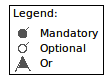
\includegraphics[width=.2\textwidth]{imagens/fm-hpl2.png}
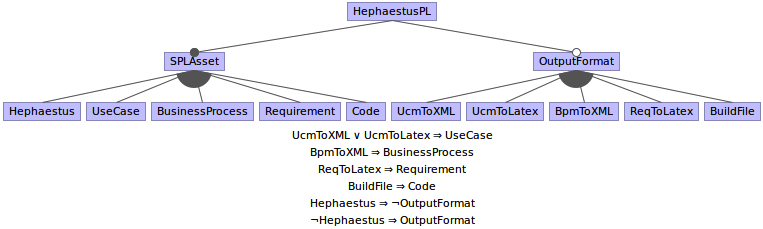
\includegraphics[width=\textwidth]{imagens/fm-hpl1.png}
\end{center}
\caption{\hpl's feature model. In this version, the features \textit{SPLAsset} and \textit{OutputFormat} define an \emph{or} relationship with their children}
\label{fig:hephaestus-fm-03}
\end{figure*}

%%%%%%%%%%%%%%%%%%%%%%%%%%%%%%%%%%%%%%%%%%%%%%%%%%

\subsection{\hpl's Feature Model} 
\label{feature-model-hpl}

In terms of the problem space, \hpl' feature model is represented in Figure~\ref{fig:hephaestus-fm-03}. As the diagram shows, the \emph{SPLAsset} feature is mandatory and the \emph{OutputFormat} feature; these features are parents of \emph{or-features} so that any combination of models and output formats is supported, e.g., a given instance might comprise business processes and use cases and export both assets as XML files. Managing variabilities in such a combination of features is essential in \hpl{} and has not been addressed elsewhere.

%%%%%%%%%%%%%%%%%%%%%%%%%%%%%%%%%%%%%%%%%%%%%%%%%%

\begin{figure*}[htb]
\begin{center}
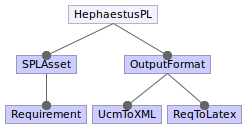
\includegraphics[scale=0.6]{imagens/confInvalid.png}
\end{center}
\caption{An invalid configuration of \hpl}
\label{fig:hephaestus-conf-invalid}
\end{figure*}

%%%%%%%%%%%%%%%%%%%%%%%%%%%%%%%%%%%%%%%%%%%%%%%%%%

In addition to the feature diagram, Figure~\ref{fig:hephaestus-fm-03} shows some cross tree constraints that must be satisfied for any valid feature configuration of \hpl.  To illustrate, Figure~\ref{fig:hephaestus-conf1a} and Figure~\ref{fig:hephaestus-conf1b} show two valid configurations of \hpl, whereas Figure~\ref{fig:hephaestus-conf-invalid} shows an invalid configuration of \hpl, in which the \emph{UcmToXML} feature is selected, but the \emph{UseCase} feature is not selected. In this case, the $UcmToXML \lor UcmToLatex \rightarrow Use Case$ constraint was violated, leading to an invalid feature configuration of \hpl.

Thus, in the problem space, a specific configuration of \hp{} is conceptually simple in that it is represented by a combination of a few \textit{or-features}. However, in the solution space, a specific configuration implies more complexity because it represents managing variability in a combination of artifacts (data types, functions of different kinds, and models) at different levels of granularity (i.e., course-grained and fine-grained), and the implementation of the features is somewhat scattered in \hp' source code.

%%%%%%%%%%%%%%%%%%%%%%%%%%%%%%%%%%%%%%%%%%%%%%%%%%

\subsection{Identification of Commonality} 
\label{commonality}

In the solution space, there exists significant amount of commonality among configurations. 
The domain analysis revealed \emph{commonality} for these abstractions across the variants of the evolution history:

\begin{itemize}

\item \emph{Feature Model Representation}: an algebraic data type represents the feature model of a product line.
  
\item \emph{Product Configuration Representation}: an algebraic data type represents a valid feature configuration.

\item \emph{Configuration Knowledge Representation} (CK Representation): an algebraic data type represents the product line's configuration knowledge.

\item \emph{Interpreter for Product Instantiation}: the \texttt{build} function performs the SPL instantiation by generating a product corresponding to a specific product line configuration.

\end{itemize}

%%%%%%%%%%%%%%%%%%%%%%%%%%%%%%%%%%%%%%%%%%%%%%%%%%

\subsection{Identification of Variability} 
\label{variability}

The domain analysis revealed \emph{variability} for these abstractions across the variants of the evolution history:

\begin{itemize}

\item \emph{Asset Representations}: algebraic data types represent the abstract syntax of different SPL assets (such as use cases, business processes, and code).

\item \emph{Asset Transformations}: functions manipulate such artifacts, solving variability of SPL assets. Some transformations basically select a specific asset from the product line, including it into the product during product derivation. Other transformations change the structure of an asset of the SPL in the final product.

\item \emph{Asset I/O}: parser/output functions for reading/writing artifacts convert the concrete syntax of an asset to/from the corresponding abstract syntax of \hpl{}, i.e., the asset abstract data types.

\item \emph{Asset Container}: the \texttt{SPLModel} and \texttt{InstanceModel} algebraic data types comprise the set of SPL assets and group it with the feature model or feature configuration, respectively, of a given \hpl{} instance.

\item \emph{Empty Instance}: an expression defines the initial representation of a product during the product derivation activity. It is an instance of the \texttt{InstanceModel} data type and serves as a baseline that is successively refined by the \texttt{build} function.

\item \emph{Configuration Knowledge Parser} (CK Parser): the \texttt{xml2Transformation} function parses the XML representation of transformations into actual transformations (functions) on instance models.

\end{itemize}

Domain analysis also substantiated that variability has a regular form that may be understood linguistically in terms of introduction of new abstractions (`modules') and extension of existing abstractions (data types and functions). For example, to introduce variability support for one new asset in \hp, one needs to implement the data types for representing the abstract syntax of these models, implement the transformations for solving variability, implement the parser and output functions for reading/writing these assets into/from \hp; one also needs to extend some data types and functions of \hp{}, as it was illustrated in Section~\ref{hp-evolution}.


%%%%%%%%%%%%%%%%%%%%%%%%%%%%%%%%%%%%%%%%%%%%%%%%%%

\section{Domain Design of \hpl}
\label{sec:domainDesign}

This section introduces the domain design~\cite{gpbook} of \hpl. We begin with an architectural view (Section~\ref{sec:hpl-architecture}). Then, we describe \hpl's transformational approach to variability management (Section~\ref{sec:hpl-transformation}), which also relies on designated configuration knowledge (Section~\ref{sec:hpl-ck}), and a derivation process for SPL tools (Section~\ref{sec:hpl-derivation}).  Finally, bootstrapping of \hpl{} is described (Section~\ref{sec:hpl-bootstrapping}).

%%%%%%%%%%%%%%%%%%%%%%%%%%%%%%%%%%%%%%%%%%%%%%%%%%

\begin{figure*}[t!]
\begin{center}
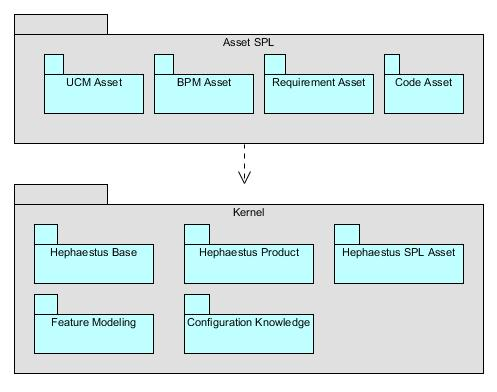
\includegraphics[width=.9\textwidth]{imagens/architecture-hpl-vf.jpg}
\end{center}
\caption{\hpl's architecture}
\label{fig:hpl-architecture}
\end{figure*}

%%%%%%%%%%%%%%%%%%%%%%%%%%%%%%%%%%%%%%%%%%%%%%%%%%

\subsection{\hpl's Architecture} 
\label{sec:hpl-architecture}

\hpl's architecture is depicted in Figure~\ref{fig:hpl-architecture}. Overall, \hpl{} is componentized in a way that most parts are separately compilable and unaffected by configuration or extension.

\emph{Kernel} represents the basic abstractions necessary for the generation of \hpl{} instances including the generation of \hpl{} itself in a bootstrapping process. Within the kernel, component \hpbase{} represents the commonality among all \hpl{} instances (as identified in Section~\ref{sec:commonality}); it serves as a base for deriving all \hpl{} instances. To this end, \hpbase{} has variability points (as identified in Section~\ref{sec:variability}) which are to be resolved by transformations defined in component \hpsplasset{} in a derivation process driven by component \hpproduct. These components of the kernel had to be specifically designed and implemented for \hpl. The kernel also hosts \emph{Feature Modeling} and \emph{Configuration Knowledge}: these components provide
basic abstractions for the representation of feature models, feature configurations, configuration knowledge as well as associated support functionality, e.g., for verifying validity of feature configurations relative to a given feature model. These components of the kernel could be reused from \hp{} and all \hpl{} instances share them, as is.

\textit{SPL Assets} represents the assets of \hpl. Each such \emph{meta-level} asset essentially corresponds to a type of artifact that can be targeted with an \hpl{} instance including the corresponding (non-meta-level) asset base for the type and designated support for variability management and product derivation in the domain of the asset. Each meta-level asset is essentially packaged in a component that exposes abstractions corresponding to the variation points of Section~\ref{sec:variability}: datatypes for the representation of assets and their transformation, functions for the interpretation of transformations, and other functionality related to \hpl's feature model, notably export functions.

%%%%%%%%%%%%%%%%%%%%%%%%%%%%%%%%%%%%%%%%%%%%%%%%%%

\subsection{\hpl's Transformational Approach} 
\label{sec:hpl-transformation}

We adopt a transformational approach to variability management. That is, the derivation of an \hpl{} instance involves source-code transformation. The approach provides transformations to address the heterogeneity of the variability patterns observed in Section~\ref{sec:hp-evolution} without compromising modularity and comprehensibility of \hpl, and thus configurability and extensibility, which may be issues for annotative approaches~\cite{kastner:2008}. The approach is also designed for uniformity. That is, the \hp{} approach to feature modeling, feature configuration, declaration and interpretation of configuration knowledge is adopted also at the meta-level. \hp{} often delegates some part of variability management to external tool support (e.g., for pre-processsing or aspect weaving), in which case, the transformation in the configuration knowledge essentially trigger those external transformations. In contrast, \hpl{} fully implements the meta-level transformations as metaprograms in Haskell on top of object programs in Haskell.

%%%%%%%%%%%%%%%%%%%%%%%%%%%%%%%%%%%%%%%%%%%%%%%%%%

\begin{figure}[t!]
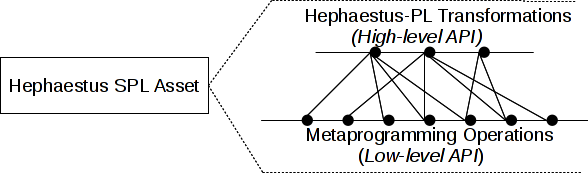
\includegraphics[scale=0.7]{imagens/apis-hpl-asset.png}
\caption{API levels for \hpsplasset}
\label{fig:hpl-apis}
\end{figure}

%%%%%%%%%%%%%%%%%%%%%%%%%%%%%%%%%%%%%%%%%%%%%%%%%%

Configuration of \hpl{} relies on transformations provided by a high-level API, which are implemented in terms of 
transformations of a low-level API, which, in turn, are implemented in terms of metaprogramming operations (with Haskell used both for object- and metaprograms).  The high-level API captures asset selection, export-format selection, and auxiliary issues, as listed below. The low-level API captures adaptation patterns as identified during the examination of the evolution scenario in Section~\ref{sec:hp-evolution}. Figure~\ref{fig:hpl-apis} illustrates the API layers, as they are part of \hpl's component \hpsplasset{} in the \emph{Kernel}. We refer to  Section~\ref{sec:metaprogrammingOperations} for the description of the actual implementation.

The transformations of the high-level API are of specific interest from the point of view of domain design, as these transformations are directly used in the configuration of \hpl. A description follows. (Some details specific to bootstrapping are deferred until Section~\ref{sec:hpl-bootstrapping}.)

\begin{description}

\item[SelectBase] selects \hpbase{}, which represents the commonality of all \hpl{} instances.
Typically, this is the first transformation to be executed in the process of deriving an instance. The implementation of \hpbase{} is given in Section~\ref{sec:hpbase}.

\item[BindProductName] sets the module name of the \hpl{} instance.

\item[SelectAsset] refines the product being derived with support for the selected asset, thereby enabling variability management for the associated type of artifacts. Technically, the transformation extends datatypes and functions for \assetr, \assetx, \asseti, \assetc, \emptyi, and \ckparser{} according to the variability identified in Section~\ref{sec:variability}. To this end, existing extension points of \hpbase{} are connected with asset-specific abstractions and the underlying modules are added to the product.

\item[SelectExport] refines the product being derived with support for the selected couple of output format and asset. To this end, the transformation extends datatypes and functions for \asseto{} in a manner very similar to \emph{SelectAsset}. 

\end{description}

%%%%%%%%%%%%%%%%%%%%%%%%%%%%%%%%%%%%%%%%%%%%%%%%%%

\begin{table}[t!]
\begin{center}
\begin{tabular}{||l||l||}
  \hline
  \textbf{Feature Expressions} & \textbf{Transformations}   \\  \hline
  True & SelectBase \\  \hline
%  Hephaestus & BindProductName "Hephaestus" \\
%             &  SelectAsset "Hephaestus"   \\
%             &  RemoveProductMainFunction \\ \hline
%  NOT Hephaestus & SelectCKParser \\ \hline
  UseCase & SelectAsset "Use Case" \\ \hline
  UseCase AND UcmToXML & SelectExport "UcmToXML"  \\ \hline
  UseCase AND UcmToLatex & SelectExport "UcmToLatex" \\ \hline
  BusinessProcess & SelectAsset "Business Process" \\ \hline
  BusinessProcess AND BpmToXML & SelectExport "BpmToXML" \\ \hline
  Requirement & SelectAsset "Requirement" \\ \hline
  Requirement AND ReqToLatex & SelectExport "ReqToLatex" \\ \hline
  Code & SelectAsset "Code" \\ \hline
  Code AND BuildFile & SelectExport "BuildFile" \\ \hline
\end{tabular}
\caption{\hpl's configuration knowledge}
\label{tab:hpl-ck}
\end{center}
\end{table}

%%%%%%%%%%%%%%%%%%%%%%%%%%%%%%%%%%%%%%%%%%%%%%%%%%

\subsection{\hpl's Configuration Knowledge} 
\label{sec:hpl-ck}

Table~\ref{tab:hpl-ck} shows \hpl's configuration knowledge, without some details related to bootstrapping, which are deferred to Section~\ref{sec:hpl-bootstrapping}.

%%%%%%%%%%%%%%%%%%%%%%%%%%%%%%%%%%%%%%%%%%%%%%%%%%

\subsection{\hpl's Derivation Process} 
\label{sec:hpl-derivation}

%%%%%%%%%%%%%%%%%%%%%%%%%%%%%%%%%%%%%%%%%%%%%%%%%%

The derivation process evaluates the condition for each line of CK for the given feature configuration. 
In this manner, transformations with true conditions are collected; they are applied consecutively in the order, as they appear in the table, with the \emptyi{} serving as input for the first transformation and the final product corresponding to the output of the last transformation. 

%%%%%%%%%%%%%%%%%%%%%%%%%%%%%%%%%%%%%%%%%%%%%%%%%%

\begin{figure*}[t!]
\begin{center}
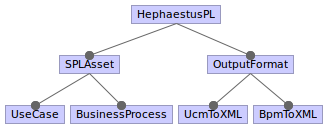
\includegraphics[scale=0.8]{imagens/fc-ucm-bpm.png}
\end{center}
\caption{An illustrative \hpl's feature configuration}
\label{fig:fc-ucm-bpm}
\end{figure*}

%%%%%%%%%%%%%%%%%%%%%%%%%%%%%%%%%%%%%%%%%%%%%%%%%%

Figure~\ref{fig:fc-ucm-bpm} shows a feature configuration which we use for the illustration of the derivation process. The configuration selects four features: use case models (\emph{UseCase}), business process models (\emph{BusinessProcess}), and both kinds models in XML format (\emph{UcmToXML} and \emph{BpmToXML}).

%%%%%%%%%%%%%%%%%%%%%%%%%%%%%%%%%%%%%%%%%%%%%%%%%%

\begin{figure*}[t!]
\begin{center}
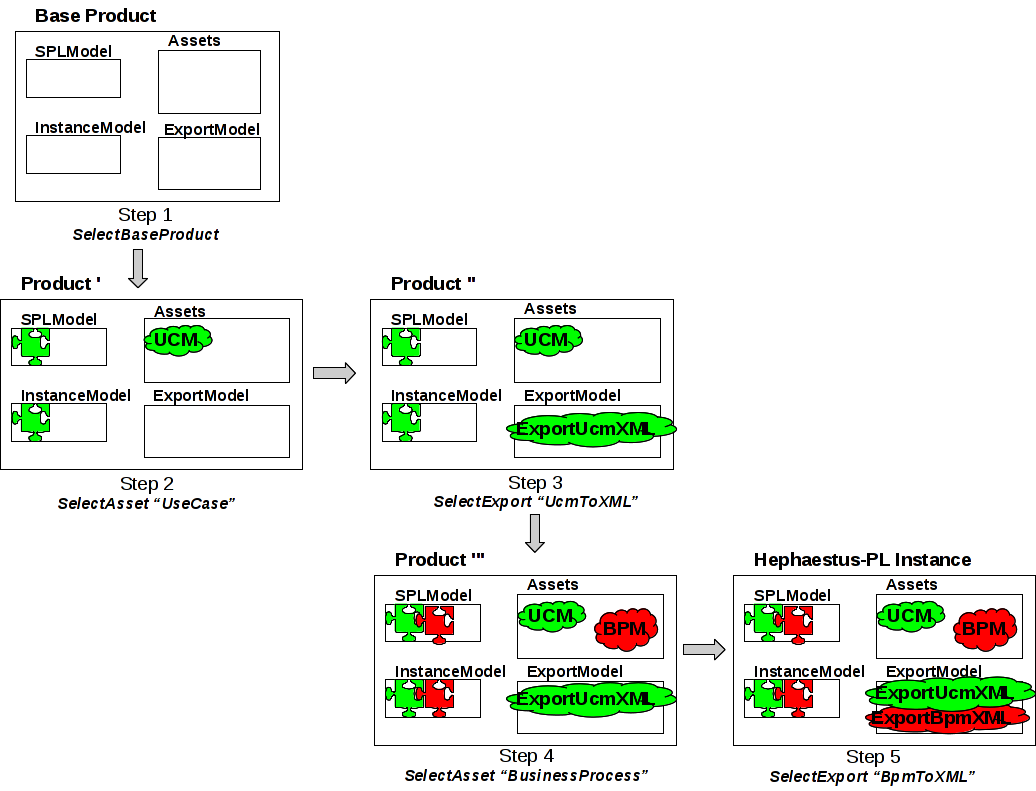
\includegraphics[width=\textwidth]{imagens/derivation.png}
\end{center}
\caption{Derivation of an \hpl{} instance supporting the UCM, BPM, UcmToXML and BpmToXML features}
\label{fig:hpl-derivation}
\end{figure*}

%%%%%%%%%%%%%%%%%%%%%%%%%%%%%%%%%%%%%%%%%%%%%%%%%%

Figure~\ref{fig:hpl-derivation} abstractly depicts the steps taken in \hpl's product derivation process 
for the feature configuration of Figure~\ref{fig:fc-ucm-bpm}. \hpl{}'s CK guides this transformational process in five steps towards the generation of a \hpl{} instance from the base product.

\hpl's product derivation process begins with the execution of the \texttt{SelectBase} transformation associated with the feature expression \texttt{True} in the first line of \hpl's CK (Table ~\ref{tab:hpl-ck}); see the first step in Figure~\ref{fig:hpl-derivation}. Next, the \emph{UseCase} feature expression in the second CK line evaluates to true for the feature configuration at hand and thus the \texttt{SelectAsset "Use Case"} transformation is executed; see the second step in Figure~\ref{fig:hpl-derivation}. In this manner, the \emph{UCM Asset} is incorporated into the product. 
Next, the \emph{UseCase AND UcmToXML} feature expression in the third CK line evaluates to true and thus the \texttt{SelectExport "UcmToXML"} transformation is executed; see the third step in Figure~\ref{fig:hpl-derivation}. In this manner, \asseto{} for the \emph{UCM Asset} is incorporated into the product. Another two steps handle the \emph{BPM Asset} very similar to the \emph{UCM Asset}.

%%%%%%%%%%%%%%%%%%%%%%%%%%%%%%%%%%%%%%%%%%%%%%%%%%

\subsection{Bootstrapping of \hpl} 
\label{sec:hpl-bootstrapping}

Consider again \hpl's architecture in Figure~\ref{fig:hpl-architecture}. \hpsplasset{} in the \emph{Kernel} provides datatypes and functions for representing and transforming \hpl{} products, i.e., tools for product derivation---in the same way as the components in the \emph{Asset SPL} provide datatypes and functions for regular assets. Thus, bootstrapping of \hpl, specifically derivation of \hpproduct, is relatively straightforward, as we discuss now.

%%%%%%%%%%%%%%%%%%%%%%%%%%%%%%%%%%%%%%%%%%%%%%%%%%

\begin{table}[t!]
\begin{center}
\begin{tabular}{||l||l||}
  \hline
  \textbf{Feature Expressions} & \textbf{Transformations}   \\  \hline
  Hephaestus & BindProductName "Hephaestus" \\
  Hephaestus & SelectAsset "Hephaestus"   \\
  Hephaestus & RemoveProductMainFunction \\ \hline
  NOT Hephaestus & SelectCKParser \\ \hline
\end{tabular}
\caption{Additional CK of \hpl{} related to bootstrapping}
\label{tab:hplck-2}
\end{center}
\end{table}

%%%%%%%%%%%%%%%%%%%%%%%%%%%%%%%%%%%%%%%%%%%%%%%%%%

\hpl's feature model contains a designated feature \hp, which is selected for bootstrapping. \hpl's configuration knowledge handles the feature in the manner shown in Table~\ref{tab:hplck-2}. The first two lines of CK directly model that bootstrapping builds \hpproduct{} from \hpsplasset.  That is, when the \hp{} feature is selected, the product name is set to be ``\hp'' and the ``\hp'' asset (i.e., \hpsplasset{} in the architecture) is selected. 

The last two lines are somewhat more idiosyncratic. The third lines models that \hpproduct{} uses a different (in fact, a much simpler) \texttt{main} function than other products. To this end, an extra transformation \emph{RemoveProductMainFunction} is invoked, with the simple intended semantics of removing the \texttt{main} for the product being derived. The fourth line models that \emph{CK parser} is only needed if features other than \hp{} are selected. To this end, an extra transformation \emph{SelectCKParser} is invoked, with the intended semantics of enhancing the product being derived such configuration knowledge is parsed, and passed as an argument to the \texttt{build} function. \hpproduct{} does not need \emph{CK Parser} because its configuration knowledge is defined as an abstraction as part of \hpsplasset; thus, parsing is not needed.

%%%%%%%%%%%%%%%%%%%%%%%%%%%%%%%%%%%%%%%%%%%%%%%%%%


\section{Implementation of \hpl}
\label{sec:implementation}


\begin{figure*}[bth]
\begin{center}
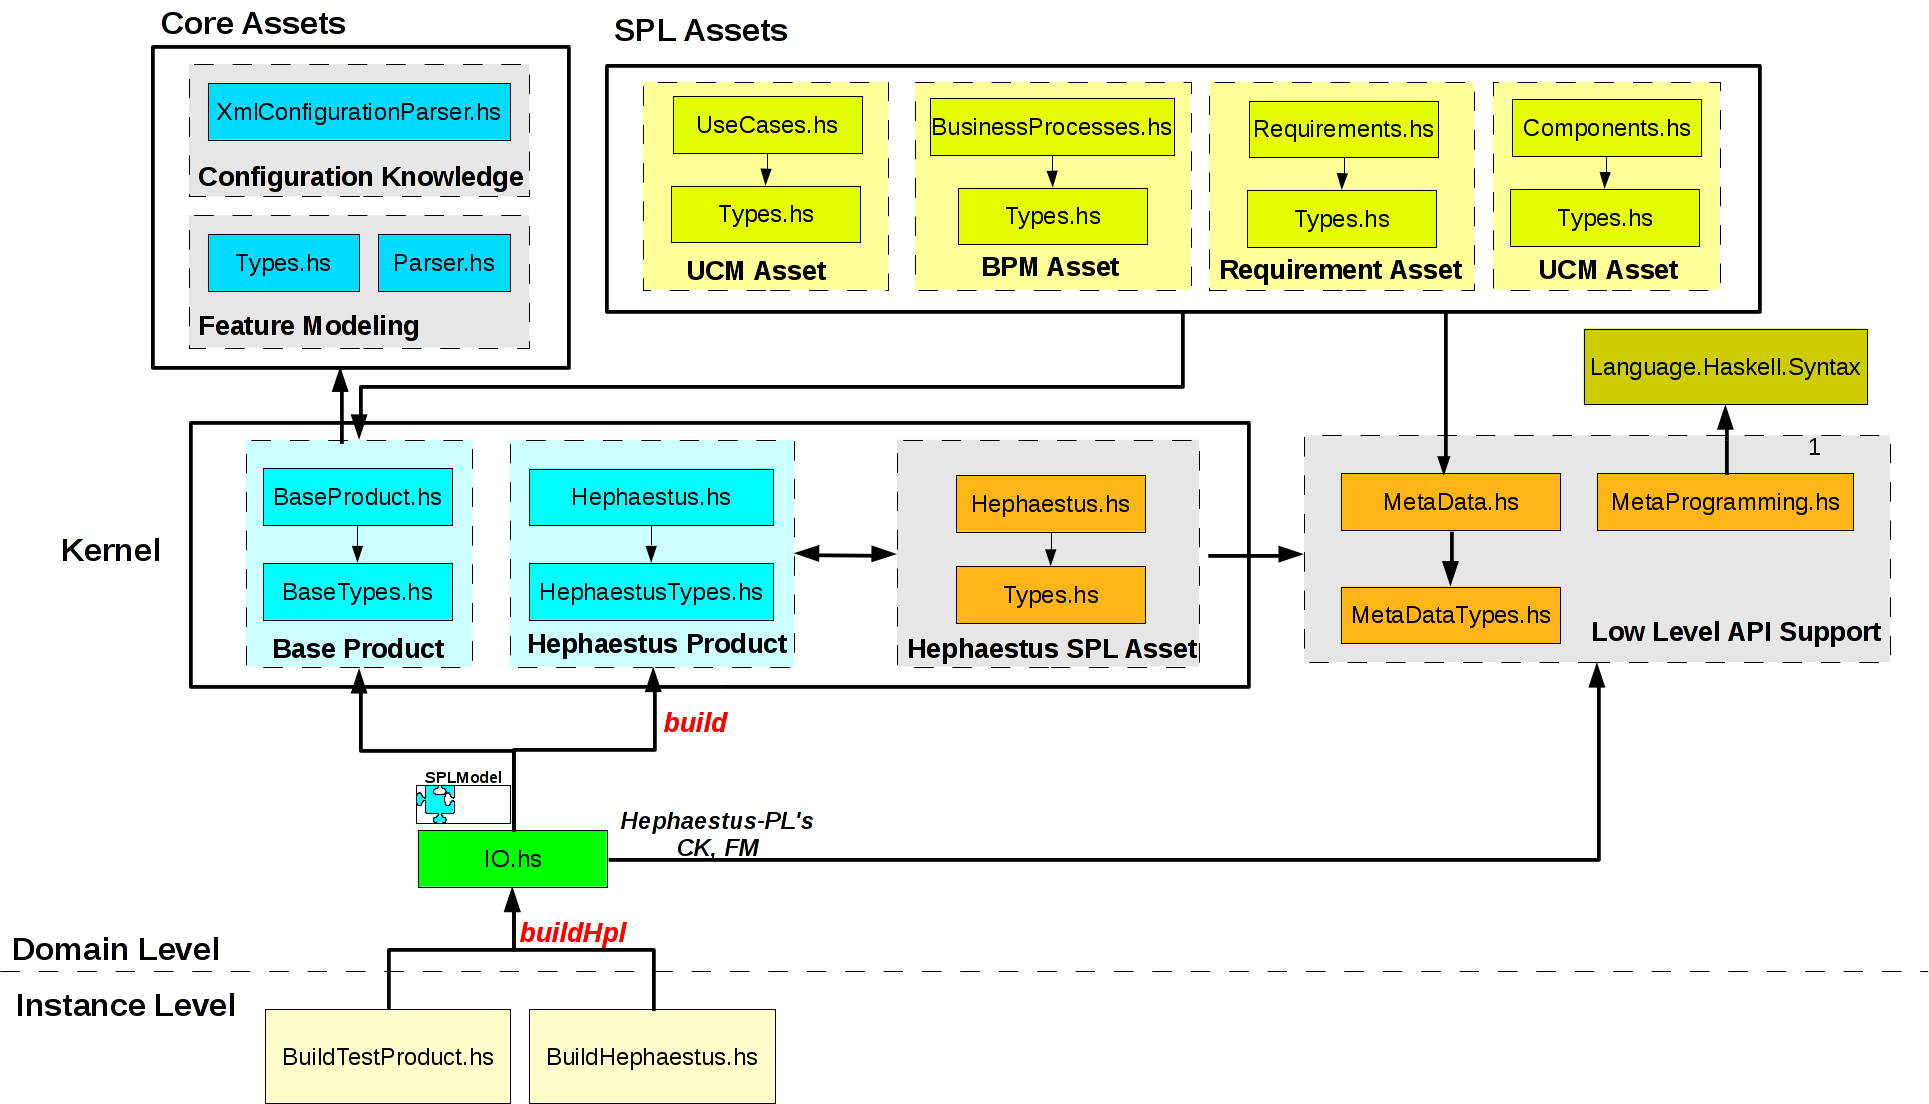
\includegraphics[scale=0.35]{imagens/modules-hpl.png}
\end{center}
\caption{Hephaestus-PL's modules dependency}
\label{fig:modules-hpl}
\end{figure*}


%\subsection{Objective of the experiment}

%The objective was to understand whether a) Haskell metaprogramming techniques can be used to obtain instances of Hephaestus that cover selected variations of assets, e.g., use cases and business processes, and b) such a metaprogramming approach can be provided in a way that the Hephaestus product-line infrastructure is applied to itself.

%\subsection{Summary of the results}

%Subject to a number of simplifying assumptions, the experiment was successfully completed. One simplification concerns the assets in scope. We used mockups as opposed to the actual implementations in Hephaestus. If we were to use the actual implementations, the relevant modules may require some changes. Another simplification concerns the feature model of Hephaestus. We only consider the OR feature for the different assets.

In this section we present the details of the implementation of \hpl's architecture shown in the Figure~\ref{fig:architecture-hpl} in terms of modules e their dependencies, as depicted in Figure~\ref{fig:modules-hpl}.
The dotted line comprises the modules which compose each of the main elements in the \hpl's architecture, i.e., the \texttt{BaseProduct.hs} and \texttt{BaseTypes.hs} modules are the \textit{Base Product} of the \hpl's Kernel.
We present the domain level's modules which support the generation of new \hpl{} intances and the instance level's modules which were developed to test \hpl{} with a selected feature configuration. Besides that, we present the metaprogramming operations which implement the transformations in Haskell code of a \textit{Base Product} of the \hp{} instance.
The source code of \hpl{} is publicly\footnote{https://gitorious.org/hephaestus-pl/hephaestus-pl} available.


\subsection{Modules and Dependencies}

At the domain level, the \texttt{IO.hs} module contains the \texttt{buildHpl} function which represents the interface to the \hpl{}'s instance level. This function is the initial point for the generation of a new \hpl{} instance by the \hpl{}'s product derivation process.  
The \texttt{buildHpl} function receives a feature configuration of \hpl{}'s FM as input and prepares the environment to execute the generation of \hpl{} instance (guided by \texttt{build} function of \textit{\hp{} Product}). 
The inputs to the derivation process of \hpl{} are four: a instance of the \texttt{SPLModel} data type, a valid feature configuration and the \hpl's FM and CK.
In this context, the instance of the \texttt{SPLModel} data type wraps the \hp{} asset, i.e., the physical modules of the \textit{\hpl{} base product} are inserted into an instance of \texttt{HephastusModel} data type that represents the abstract type of \hp{} asset and it is wrapped into an \texttt{SPLModel} data type. 
Besides, the derivation process of \hpl{} needs the \hpl{}'s feature modeling and configuration knowledge
%has the goal of preparing the elements (\texttt{SPLModel} data type, feature modeling and configuration knowledge) of \hp{} 
to execute the \texttt{build} function of the \textit{\hp{} Product} that controls the generation of the new \hpl's instance. 
The \hpl's FM and CK are contained into \texttt{MetaData.hs} module. Then, 
%Thus, are selected the \textit{Base Product's} modules which represent the \texttt{HephastusModel} data type and are inserted into \texttt{SPLModel} data type and are selected the \hpl's FM and CK contained into \texttt{MetaData.hs} module to call 
the \texttt{build} function contained into \texttt{\hp.hs} module (\textit{\hp{} Product}) is executed and returns the new \hpl{} tool instance. 
Therefore, the \texttt{IO.hs} module depends of \textit{Base Product's} modules, \textit{\hp{} Product's} modules and \texttt{MetaData.hs} module, as shows the Figure~\ref{fig:modules-hpl}.

The \textit{\hp{} Product's} modules depend strongly on \textit{\hp{} SPL Asset's} modules that implement the \texttt{HephaestusModel} and \texttt{HephaestusTransformation} data types and \texttt{transformHpl} function, i.e., the \texttt{build} function evaluates the CK and calls the \texttt{transform} function defined in the same \hp.hs module into \textit{\hp{} Product} that executes the \texttt{transformHpl} function into \hp.hs module of \textit{ \hp{} SPL Asset} to solve the \hpl{} transformation.

The \texttt{MetaData.hs}, \texttt{MetaDataTypes.hs} and \texttt{MetaProgramming.hs} modules comprise the group called \textit{Low Level API Support} that implement the metaprogramming operations to solve the variation points in \textit{Base Product's} modules. The \texttt{MetaProgramming.hs} module depends the Language.Haskell.Syntax package.

The \textit{SPL Assets} are composed by pairs of modules: the \texttt{Types.hs} module which defines the algebraic data types of the asset to insert into \texttt{SPLModel} and \texttt{InstanceModel} data types of \hpl{} instance and defines the data types which are used as constructors into \texttt{TransformationModel} and \texttt{ExportModel} data types of \texttt{BaseTypes.hs} module. 
Besides, another module (\texttt{assetName.hs}) of each group in \textit{SPL Assets} defines the functions which are used into \texttt{transform}, \texttt{mkEmptyInstance} and \texttt{export} functions of \texttt{BaseProduct.hs} module. Thus, the \textit{SPL Assets} modules depend the \textit{Base Product's} modules.

Finally, we have the \textit{Core Assets'} modules (FM and CK) that are imported by \textit{Base Product's} modules.



\subsection{Description of the Transformational Approach}

The underlying hypothesis is that certain key types and functionality of any specific Hephaestus instance can be derived by metaprogramming. To this end, we consider an \texttt{Base Product} from which to build ``\hpl{} products''. All products are expected to define \texttt{SPLModel}, \texttt{InstanceModel}, \texttt{ConfigurationKnowledge}, \texttt{TransformationModel}, \texttt{ExportModel}, a transformation function \texttt{transform}, a output format function \texttt{export} and \texttt{main} function that controls the generation the product instances.

All forms of assets are hence provided in a form that they can contribution to the above-mentioned entities as presented in SPL Asset block in Figure~\ref{fig:modules-hpl}. We use metaprogramming operators that build the product's entities (say, types and functions) from the corresponding parts of the asset-related modules by adding parts incrementally to the base product.

Because of the objective of self-application of Hephaestus (bootstrapping design principle), the above-mentioned transformational approach is actually packaged as another kind of asset: Hephaestus SPL Asset. That is, the construction of any specific Hephaestus instance is controlled by a feature configuration relative to \hpl's feature model and the corresponding configuration knowledge as presented in module \texttt{MetaData.hs}.


\subsection{Metaprogramming Operations} \label{sec:metaprogrammingOperations}

\begin{table}[h]
%\begin{tabular}{||l||l||}
\begin{tabular}{ | l | p{7cm} |}
  \hline
  \textbf{\hpl{} Transformations}            & \textbf{Metaprogramming Operations}  \\  \hline
  \multirow {9} {*} {\textit{SelectAsset assetName}} & addUpdateCase \\ \cline{2-2}
                                             & initializeFieldWithFun \\ \cline{2-2}
                                             & addImportDecl (4x) \\ \cline{2-2}
                                             & addLetInstruction \\ \cline{2-2}
                                             & addGeneratorInstruction \\ \cline{2-2}
                                             & initializeField  \\ \cline{2-2}
                                             & addField (2x)  \\ \cline{2-2}
                                             & addConstructor  \\ \cline{2-2}
                                             & addUpdateCaseList \\  \hline
 \multirow {4} {*} {\textit{SelectExport assetFormat}} & addUpdateCase  \\ \cline{2-2}
                                               & addImportDecl  \\ \cline{2-2}
                                               & addConstructor \\ \cline{2-2}
                                               & addListElem \\ \hline
 \multirow {2} {*} {\textit{SelectBaseProduct}} & setModuleName (2x)  \\ \cline{2-2}
                                     & removeImportDecl \\ \hline
 \textit{BindProductName}            & setModuleName (2x)  \\ \hline
 \textit{RemoveProductMainFunction}  & removeFunction \\ \hline
 \multirow {3} {*} {\textit{SelectCKParser}}  & addImportDecl \\ \cline{2-2}
                                     & addGeneratorInstruction  \\ \cline{2-2}
                                     & addLetInstruction (2x) \\ \hline
\end{tabular}
\caption{Mapping of \hpl{} transformations into metaprogramming operations}
\label{tab:map-transformations-hpl}
\end{table}


%  \multirow {\textit{SelectAsset assetName}} & addUpdateCase & extends \textit{transform} function \\ \cline{2-3}
% & initializeFieldWithFun & initialize \textit{InstanceModel} with empty asset \\ \cline{2-3}
% & addImportDecl & import modules data types, transformations and parser of asset \\ \cline{2-3}
% & addLetInstruction & update \textit{main} function ... \\ \cline{2-3}
% & addInstructionGenerator & insert asset's parser function in \textit{main} function \\ \cline{2-3}
% & initializeField & update SPLModel data type in \textit{main} function \\ \cline{2-3}
% & addField & insert asset data type in \textit{SPLModel} and \textit{InstanceModel} data types \\ \cline{2-3}
% & addConstructor & insert asset transformation data type in \textit{TransformatonModel} data type \\ \cline{2-3}
% & addParserCKList & insert asset transformation names in \textit{xml2Transformation} function \\  \hline
% \multirow {\textit{SelectExport assetFormat}} & addUpdateCase & extends \textit{export} function \\ \cline{2-3}
% & addImportDecl & import asset output format module \\ \cline{2-3}
% & addConstructorWithoutArgs & insert asset output format data type in \textit{ExportModel} data type \\ \cline{2-3}
% & addElemList & insert asset output format data type in \textit{lstExport} list \\ \hline
% \textit{SelectBaseProduct}} & setModuleName & rename the \hpl{} instance module from "BasicProduct" to "Test" \\ \cline{2-3}
% & removeImportDecl & \\ remove the line \texttt{import HplProducts.EmptyTypes} from \hpl{} instance module \cline{2-3}
% & addImportDecl & \\ \cline{2-3}
% & addInstructionGenerator & \\ \hline
% \textit{BindProductName}} & setModuleName &  \\ \hline


The required metaprogramming operations are of different complexity as implemented in \texttt{MetaProgramming.hs} module. We begin with the simpler operations. There is an operation \texttt{setModuleName} to modify the module name so that the module of the base product can be renamed into a module for the emerging product, say \hp{} instance. This operation is performed on the \texttt{SelectBaseProduct} and \texttt{BindProductName} transformations.
There is an operation \texttt{addImportDecl} to add an import declaration to the main module of the emerging product; this operation is needed to incorporate any additional kind of asset. This operation is performed on the \texttt{SelectCKParser} transformation to add an import declaration to CK parser (\texttt{CK.Parsers.XML.XmlConfigurationParser} module); on the \texttt{SelectAsset} transformation to add import declarations to incorporate the asset modules (algebraic data types, transformations, parser and output format) and the data types module of emerging product.
There is an operation \texttt{addField} to extend a given record type with a field; this operation is needed in the extension of Hephaestus' data types \texttt{SPLModel} and \texttt{InstanceModel}.
There is also an operation \texttt{addConstructor} to extend a given algebraic data type with a constructor declaration besides to remove the constructor declaration not used, i.e., \texttt{UndefinedTransformation} constructor; this operation is needed for assembling Hephaestus' data type \texttt{TransformationModel} for transformations on possibly different forms of assets. We note here that \texttt{addConstructor} is deliberately limited to only support the addition of a constructor with a single constructor component and to actually reuse that component's specified type for the constructor's name.
Therefore, we defined a similar operation \texttt{addConstructorWithoutArgs} to extend the Hephaestus' data type \texttt{ExportModel} for different asset output formats. In this case, the \texttt{addConstructorWithoutArgs} only supports the addition of a constructor's name without components. We also remove the variation point declaration \texttt{UndefinedExport} in this operation.
The operation \texttt{addListElem} adds into \texttt{lstExport} list the constructors of the Hephaestus' data type \texttt{ExportModel}.

The addition of fields and constructors is relatively straightforward at the type level, but we need additional, non-trivial operations that transform functions that readily use the affected types. There are the operations \texttt{initializeField} and \texttt{initializeFieldWithFun} which modify all expressions for record construction for a given record type such that in the first case a given field is initialized by a constant (say, a variable name or a function name with assumed zero arity) and in the second case a given field is initialized by a function name with assumed one arity, i.e., the empty asset function that receives the asset data type as input parameter. Other forms of reaction to added fields are conceivable, but the given form turned out to be sufficient in the experiment.
There is also an operation \texttt{addUpdateCase} which extends function definitions by a case in reply to a previously added constructor. Different forms of adding cases are conceivable. The following, non-trivial form was required in the experiment.

Addition of a constructor is needed for \texttt{TransformationModel}, which in turn is to be used in a \emph{transform} function that essentially interprets transformation models (`terms'). The type of the function is this:

\begin{lstlisting}
transform :: TransformationModel
          -> SPLModel
          -> InstanceModel
          -> InstanceModel
\end{lstlisting}

The idea is here that the function perhaps case discrimination on the \emph{first} argument and essentially delegates to a more specific transformation function that readily handles the given transformation on the further arguments at hand. An additional complication arises from the fact that the more specific transformation function would not be able to operate on the composed types \texttt{SPLModel} and \texttt{InstanceModel}. For example, consider a Hephaestus instance that should support use cases and business processes. Then, the following \texttt{transform} function has to be synthesized:

\begin{lstlisting}
transform (UseCaseTransformation x0) x1 x2 = transformUcm  x0 x1 x2
transform (BusinessProcessTransformation x0) x1 x2 = transformBpm  x0 x1 x2
\end{lstlisting}

Hence, the  operation \texttt{addUpdateCase} must add cases such that indeed case discrimination is performed on the first argument and the last two arguments are defined by \texttt{x1} and \texttt{x2} variables when being passed to the function on the RHS.
A similar operation to \texttt{addUpdateCase} was defined to extend the \texttt{export} function definition by a case in reply to a previously added constructor into \texttt{ExportModel} data type. The type of the function is this:

\begin{lstlisting}
export :: ExportModel -> FilePath -> InstanceModel -> IO ()
\end{lstlisting}

For example, consider a Hephaestus instance that should support use cases and business processes in xml format. Then, the following \texttt{export} function has to be synthesized:

\begin{lstlisting}
export :: ExportModel -> FilePath -> InstanceModel -> IO ()
export (ExportUcmXML) x1 x2  = exportUcmToXML (x1 ++ ".xml") (ucm x2)
export (ExportBpmXML) x1 x2  = exportBpmToXML (x1 ++ ".xml") (bpm x2)
\end{lstlisting}

The extension of the \texttt{xml2Transformation} function is also done with the \texttt{addUpdateCase} operation applied in a list of cases of transformations supported by CK for the emerging \hpl{} product.


Moreover, we defined two new operations to extend the \texttt{main} function into a module for the emerging product, they are \texttt{addLetInstruction} and \texttt{addGeneratorInstruction}. The first is used to add  \texttt{let} sentences in the \texttt{main} function to recover the asset spl and to execute the parser function and moving the asset spl into \hpl's instance. The second operation \texttt{addGeneratorInstruction} is used to add instructions about asset and CK parsers into module for the emerging product.
The operation \texttt{addLetInstruction} adds the instruction \texttt{let product = build fm fc cm spl} responsable for generation of new \hpl's instances. To ensure the compilation of BaseProduct and \hpl{} modules, we add the instructions related to CK (import and parser) and the calling of \texttt{build} function only in emerging product.

There is also the \texttt{addUpdateCaseList} operation based on \texttt{addUpdateCase} operation and using a list of cases to extend the \texttt{xml2Transformation} function that comprises the CK parser process performing the recognition of the concrete syntax of asset transformations of the \hpl{} instance.

Finally, the operation \texttt{removeImportDecl} removes an import declaration of the main module of the emerging product. This operation is performed on the \texttt{SelectBaseProduct} transformation to remove the import declaration of the module with algebraic data types of base product. This is replaced by import declaration of module with algebraic data types of emerging \hpl{} product.

The operation \texttt{removeFunction} removes the \texttt{main} function of the emerging product. It is necessary in the generation of \hp{} product because its \textit{main} function is the \texttt{builHpl} function located into \texttt{IO.hs} module. This operation is executed by \texttt{RemoveProductMainFunction} transformation assigned to \texttt{Hephaestus} expression feature.

Table~\ref{tab:map-transformations-hpl} summarizes the mapping of \hpl{} transformations into metaprogramming operations.


%\subsection{Testing the implementation}

%The experiment is provided by a self-contained directory \emph{meta-hephaestus} that is added to a master of Hephaestus as obtained from git. The following cabal packages were required: \emph{funsat-0.6.0} (as required by Hephaestus anyway) and \emph{haskell-src-1.0.1.3} (needed for metaprogramming).

%There are the following files and directories:

%\begin{itemize}

%\item File \emph{Makefile}: build and test various products.

%\item Directory \emph{doc}: this documentation.

%\item Directory \emph{HplAssets}: the asset base of the Hephaestus product line.

%\item Directory \emph{HplProducts}: products built with the Hephaestus product line.

%\item Directory \emph{HplDrivers}: Main modules to initiate building or loading.

%\end{itemize}

%Just run ``make test'' to exercise all building and loading.



%\subsection{Future work}

%\begin{itemize}

%\item The experiment does not properly support existing forms of assets such as use cases, process models, etc. Additional complexities are likely to arise when moving from mockups to real code.

%\item Additional features such as import from and export to different formats or GUI support have not been considered. Additional complexities will arise. In particular, additional metaprogramming support may be required.

%\item The product derivation is naive in so far that relevant forms of assets are simply imported by irrelevant forms are not removed. That is, Hephaestus instances would contain much `dead code'. This would be easily addressed by refining the metaprogramming approach to take care of the modules that need to be physically included into the final product. (Alternatively, a post-processing approach for dead-code elimination could be applied.)

%\item The metaprogramming operations are just implemented up to a level of proof of concept. For instance, they may have issues with variable capture.

%\item Static correctness of the Hephaestus product line has not been addressed. It would be possible though for a feature model such as Hephaestus' one to exhaustively construct all products and check them with the Haskell system.

%\item Alternative approaches may need to be investigated. For instance, we could consider pre-processing, CIDE, Feature House, or the use of type classes.

%\end{itemize}


\subsubsection{Hephaestus UCM and BPM instance's Haskell module}

%After building an \hpl{} instance,
From the \hp{} product presented in Section~\ref{hephaestus-product}, the product derivation process generates a
new Haskell module that refines the \texttt{BaseProduct} module with the
selected features of the product configuration. 
For instance, Figure~\ref{fig:code-hp-ucm-bpm} shows the \hpl{} instance source code generated by selection the features \texttt{Use Case}, \texttt{Business Process}, \texttt{UcmToXML} and \texttt{BpmToXML}. 
New cases related to these assets and output formats will be introduced into the definition of the
\texttt{transform} (lines \ref{inst-hpl-transform-function-i}-\ref{inst-hpl-transform-function-f}) and
\texttt{export} (lines \ref{inst-hpl-exportmodel-function-i}-\ref{inst-hpl-exportmodel-function-f}) functions,
as well as new data fields are introduced into the definitions of the
\texttt{SPLModel} (lines \ref{inst-hpl-splmodel-decl-i}-\ref{inst-hpl-splmodel-decl-f}),
\texttt{InstanceModel} (lines \ref{inst-hpl-instancemodel-decl-i}-\ref{inst-hpl-instancemodel-decl-f}),
\texttt{TransformationModel} (lines \ref{inst-hpl-transformodel-decl-i}-\ref{inst-hpl-transformodel-decl-f})
and \texttt{ExportModel} (line \ref{inst-hpl-exportmodel-decl}) data types,
the \texttt{mkEmptyInstance} (lines \ref{inst-hpl-instancemodel-empty-i}-\ref{inst-hpl-instancemodel-empty-f}) function returns an instance model with new data fields and, finally, new elements corresponding to \texttt{ExportModel} data type are introduced into the \texttt{lstExport} (line \ref{inst-hpl-lstexport-decl}) list.

Moreover, the \hpl{} product derivation process introduces sentences in the \texttt{main} function for
\texttt{Use Case} and \texttt{Business Process} asset parser (lines \ref{inst-hpl-asset-parser-i}-\ref{inst-hpl-asset-parser-f}) and updates the fields of the \texttt{SPLModel} instance into
\texttt{spl} (line \ref{inst-hpl-splmodel-main}) declaration and the
\texttt{product} (line \ref{inst-hpl-build-main}) declaration with calling \texttt{build} function.
%(see code snippet in the Figure~\ref{fig:code-hp-ucm-bpm}). 
Besides the mentioned transformations applied to the
\texttt{BaseProduct} module during the product derivation, the
resulting module also has to import declarations that are specific for a given
selection of features.

\begin{figure}
\begin{lstlisting}
data SPLModel = SPLModel {
  featureModel :: FeatureModel,
  splUcm :: UseCaseModel,        *'\label{inst-hpl-splmodel-decl-i}'*
  splBpm :: BusinessProcessModel *'\label{inst-hpl-splmodel-decl-f}'* 
}

data InstanceModel = InstanceModel {
  featureConfiguration :: FeatureConfiguration,
  ucm :: UseCaseModel,        *'\label{inst-hpl-instancemodel-decl-i}'*
  bpm :: BusinessProcessModel *'\label{inst-hpl-instancemodel-decl-f}'* 
} deriving (Data, Typeable)

data TransformationModel = UseCaseTransformation UseCaseTransformation                  *'\label{inst-hpl-transformodel-decl-i}'*
                         | BusinessProcessTransformation BusinessProcessTransformation  *'\label{inst-hpl-transformodel-decl-f}'*

transform :: TransformationModel -> SPLModel -> InstanceModel -> InstanceModel
transform (UseCaseTransformation x0) x1 x2 = transformUcm x0 x1 x2         *'\label{inst-hpl-transform-function-i}'*
transform (BusinessProcessTransformation x0) x1 x2 = transformBpm x0 x1 x2 *'\label{inst-hpl-transform-function-f}'*

mkEmptyInstance :: FeatureConfiguration -> SPLModel -> InstanceModel
mkEmptyInstance fc spl = InstanceModel {
  featureConfiguration = fc,
  ucm = emptyUcm (splUcm spl), *'\label{inst-hpl-instancemodel-empty-i}'*
  bpm = emptyBpm (splBpm spl)  *'\label{inst-hpl-instancemodel-empty-f}'*
}

data ExportModel = ExportUcmXML | ExportBpmXML *'\label{inst-hpl-exportmodel-decl}'*

export :: ExportModel -> FilePath -> InstanceModel -> IO ()
export (ExportUcmXML) x1 x2 = exportUcmToXML (x1 ++ ".xml") (ucm x2) *'\label{inst-hpl-exportmodel-function-i}'*
export (ExportBpmXML) x1 x2 = exportBpmToXML (x1 ++ ".xml") (bpm x2) *'\label{inst-hpl-exportmodel-function-f}'*

lstExport :: [ExportModel]
lstExport = [ExportUcmXML, ExportBpmXML]  *'\label{inst-hpl-lstexport-decl}'*

main :: IO ()
main = do
  ...
  let bModel    = fromJust (findPropertyValue "businessprocess-model" ps) *'\label{inst-hpl-asset-parser-i}'*
  let uModel    = fromJust (findPropertyValue "usecase-model" ps)
  (Core.Success bppl) <- parseBusinessProcess (ns bpSchema) (snd bModel)
  (Core.Success ucpl) <- parseUseCaseFile (ns ucSchema) (snd uModel)   *'\label{inst-hpl-asset-parser-f}'*
  let spl = SPLModel{featureModel = fm, splUcm = ucpl, splBpm = bppl} *'\label{inst-hpl-splmodel-main}'*
  let product = build fm fc cm spl   *'\label{inst-hpl-build-main}'*
  let out = (outputFile (snd targetDir) (snd name))
  sequence_ [export x out product | x <- lstExport]
\end{lstlisting}
\caption{Code snippet of the Hephaestus UCM and BPM instance}
\label{fig:code-hp-ucm-bpm}
\end{figure}






\section{Reactive Process}
\label{sec:process}

As discussed earlier, the design of \hpl{} should improve the flexibility to introduce 
support for managing variabilities on new SPL assets, and thus evolve the configurability 
space of \hpl{}. In this section we describe a process (Figure~\ref{fig:process} shows the corresponding BPMN diagram) that could guide domain engineers to proceed in this task. 
It is important to note that we have designed this process based on our experience for 
evolving the versions of \hpl{} to support several assets (use cases, business processes, requirements and code). Therefore, it focuses on the reactive process to introduce new asssets into \hpl. 

Three roles contribute to this process, which are represented as the lanes in Figure~\ref{fig:process}. Customers start the reactive 
process in \hpl{} demanding a Hephaestus tool with new requirements. Application engineers consider the new requirements,
specify and map the requirements for the features of \hpl{}, and evaluate whether the requirements are 
already supported by \hpl. If so, they generate the \hpl{} product with the desired configuration, 
testing and delivering it to the customer. If \hpl{} does not support the customer tool's requirements yet, the application 
engineers submit to the domain engineer the demand for evolving \hpl{} to support the new requirements (assets).

The domain engineers here comprise two distinct roles: \emph{asset domain expert} that defines and 
implements the artifacts of the new assets; and \emph{domain engineer of \hpl{}} that evaluates the impact and integrates the artifacts 
of the new asset into \hpl. The \emph{asset domain expert} executes activities concerning the new artifact, by providing its implementation in terms of data types, transformations, parsers, and output format functions. It corresponds the 
\textit{Define asset type structures}, \textit{Define asset transformations}, \textit{Implement asset parser} and \textit{Implement asset output format} activities in Figure~\ref{fig:process}.
No order is specified among these tasks because they are normally 
carried out iteratively. The \textit{domain engineer of \hpl{}} assesses whether the introduction of a new asset needs to update the \hpl{} 
Kernel's APIs (high and low level transformations); integrates the new asset's artifacts into \hpl{} infrastruture; updates the metadata strutures inserting references to the new 
asset; updates Hephaestus-PL's FM and CK using the guidance of safe evolution templates of software product 
lines defined~\cite{gpce11}; and validates the new asset by generating a new \hpl{} product with the selected new asset and checking 
the correctness of the generated source code. If the generated product is a valid Hephaestus product 
then the domain engineer's activities are finalized.

%This lane involves activities concerning the new artifact, i.e., providing its implementation in terms of data types, their transformations, parsers, and output format functions. No order is specified since these are normally carried out in a iterative fashion. 
%The first activity of the field engineer to evaluate the impact of HPL to support the new asset.

%In addition to these activities, this lane involves other activities to integrate the new asset to the \hp{} product line, how to introduce new modules implemented to new artifact into \hpl's infrastructure, update Hephaestus-PL's FM and CK using the guidance of safe evolution templates of software product lines defined in ~\cite{gpce11} and update the asset meta data structures that support the metaprogramming operations to manage the variability of \hpl.
%Finally, it is necessary to execute the derivation of a simplified \hpl{} product with only the new asset to validate the evolution of \hpl{}. If the generated product is a valid Hephaestus product then the domain engineer's activities are finalized. The validation of Hephaestus product can be done using a checklist. Otherwise, if the generated product is not valid or does not meet the specification of the new asset, additional activities are conducted by the domain engineer to assess possible needs for changes in the metaprogramming operations, in the asset meta data structures or in the contents of the meta data structures of the new asset until deriving a valid product.


%The lane corresponding to the domain engineer involves activities concerning the new artifact, i.e., providing its implementation in terms of data types, their transformations,  parsers, and output format functions. No order is specified since these are normally carried out in a iterative fashion. The lane corresponding to the application engineer involve integrating new modules implemented to new artifact into \hpl's infrastructure, and correspondingly updating its feature model, configuration knowledge, and asset meta data structures.
%Then,  it is necessary to execute the derivation a product with the new asset to validate the evolution of Hephaestus-PL. If the result is a valid Hephaestus product then the reactive process is finalized. The validation of Hephaestus product can be done using a checklist. Otherwise, the domain engineer analyses the errors or improper behavior of generated product Hephaestus instance and execute a set of activities to correct the error with possible needs for changes in the operations of metaprogramming and in the asset meta data structures. After that, we execute the test of the generation of an Hephaestus instance with the new asset again and we need to execute a regression test to validate that changes made in metaprogramming and in the asset meta data structures did not impact the generation of products with the assets already owned the Hephaestus-PL.

\subsection{Evolution of Hephaestus-PL to support the Requirement Model asset} \label{sec:evolHplReq}

To illustrate the execution of the reactive process we apresent the evolution of Hephaestus-PL's to support the management of variabilities in the \textit{Requirement Model} asset. The current version of \hpl{} supports \textit{Use Case Model} and \textit{Business Process Model} assets. Figure~\ref{fig:evol-hpl-req} summarizes this scenario of evolution of \hpl{} which we describe below.


\begin{figure*}[bth]
\begin{center}
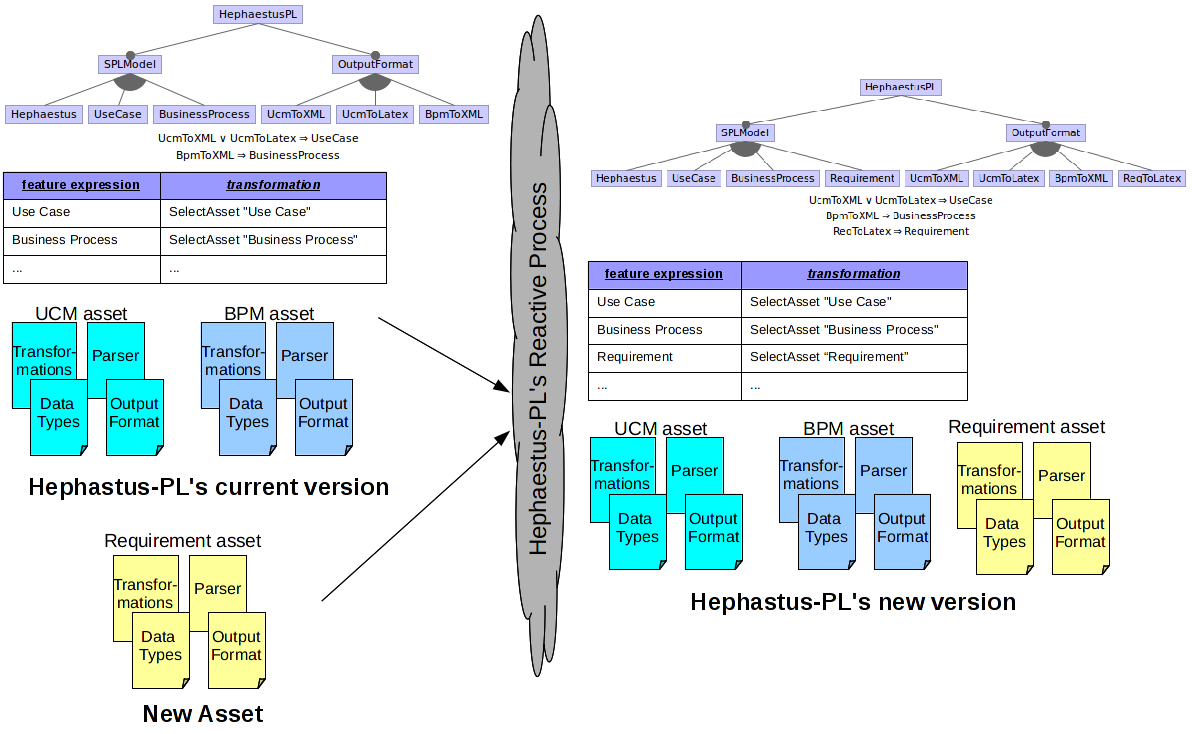
\includegraphics[scale=0.5]{imagens/evol-hpl-req.png}
\end{center}
\caption{Hephaestus-PL's Evolution to introduce the \textit{Requirement} asset.}
\label{fig:evol-hpl-req}
\end{figure*}

%The first release of \hpl{} only supports \textit{use case (UCM)} asset. 
%But, the customer requests a new \hp{} tool that supports BPM product lines. In this case, the customer defining the tool's requirements, i.e., \textit{deriving products of BPM product lines}. 
%Given the need to introduce supporting for Requirement, new requirements for the product line were provided. Because this version of \hpl{} did not support these requirements, there is a need to evolve it to support the management of variabilities in a new asset (BPM).

%The application engineer tries to map this requirement to a feature of Hephaestus-PL's FM and evaluates that \hpl{} has not supported this requirement yet. Then the application engineer submits to the domain engineer a demand for evolution of \hpl{} supporting the new requirement (BPM asset). At first in this level, 

The reactive process to introduce new assets into \hpl{} begins with the \textit{domain engineer} assessing the impacts in Kernel's APIs of \hpl{} to support the \textit{Requirement} asset. It's necessary to analyze whether the high level APIs \--- corresponding to Hephaestus-PL's transformations (\textit{SelectAsset} and \textit{SelectExport}) \--- and low level APIs \--- corresponding to the metaprogramming operations \--- support the specification of new \textit{Requirement} asset. This reactive process considers that the transformations of \hpl{} (\textit{SelectAsset} and \textit{SelectExport}) support new assets, i.e., 
%usually there will be no impact on high-level APIs in \hpl. 
based on our experience, introducing support for variation in a new asset in \hpl{} does not impact the high level APIs. 
%However, the low level APIs may require some adjustments to satisfy the new asset but it represents lower impact. In this case, both the Kernel's APIs support the \textit{Requirement} asset. 

Then, the \textit{asset domain expert} has to implement the four artifacts of \textit{Requirement} asset to evolve \hpl{} supporting this asset. The items below describe what is necessary to define about the new \textit{Requirement} asset:

\textit{(i)} to define the \texttt{RequirementModel} data type and other auxiliary types that represent a set of requirements with their variabilities. The \\ \texttt{RequirementModel} data type is composed by id, name, and description fields (see code snippet in Figure~\ref{fig:code-req-data-type}) and is located in a specific module, i.e., \texttt{ HplAssets.ReqModel.Types.hs} module; 

\begin{figure}
%\begin{code}
\begin{lstlisting}
data Requirement = Requirement {
      reqId :: Id, 
      reqName :: String,
      reqDescription :: String
} deriving (Show, Data, Typeable)        
             
data RequirementModel = RM {
      reqs :: [Requirement]
} deriving (Show, Eq, Data, Typeable)
\end{lstlisting}  
\caption{Definition of \texttt{RequirementModel} data type}
\label{fig:code-req-data-type}
%\end{code}
\end{figure}   


\textit{(ii)} to define the transformations and empty instance function of \textit{Requirement} asset. The transformations specified that managing variabilities in Requirements are \texttt{SelectAllRequirements}, \texttt{SelectRequirements} and \texttt{RemoveRequirements}. The \texttt{emptyReq} is the function which defines a Requirement asset empty instance. It is also necessary to define a data type and a function to comprise all the transformations of Requirement asset to introduce them in a product \hpl{} instance. For example, we defined the \texttt{RequirementTransformation} data type and the \texttt{transformReq} function, respectively. The definition \texttt{RequirementTransformation} must have the clause \texttt{deriving (Show, Eq, Ord)} to allow the ordering and viewing of the Requirement asset's transformations. All definitions of data types to \textit{Requirement} asset must be in \texttt{HplAssets.ReqModel.Types.hs} module. The \texttt{transformReq} function must to have a similar signature of the \texttt{transform} function into \texttt{BaseProduct.hs} module that is a \hpl{} base instance. Besides, a \texttt{transformReq} function must be defined by pattern matching for each constructor declared in the \texttt{RequirementTransformation} data type (see code snippet in Figure~\ref{fig:code-req-transf}).
Both the \texttt{emptyReq} and \texttt{transformReq} functions are implemented in a specific module, i.e., 
\texttt{ HplAssets.Requirements.hs} module. 
These functions must be visible by the \hpl{} kernel to be able to generate a new \hpl{} instance with selected \textit{Requirement} asset; 

\begin{figure}
%\begin{code}
\begin{lstlisting}
data RequirementTransformation = SelectAllRequirements 
                               | SelectRequirements [Id]
                               | RemoveRequirements [Id]
                               deriving (Show, Eq, Ord)
			       
emptyReq :: RequirementModel -> RequirementModel
emptyReq reqmodel = reqmodel { reqs = [] }

transformReq :: RequirementTransformation 
             -> SPLModel 
             -> InstanceModel 
             -> InstanceModel
             
transformReq (SelectAllRequirements) spl product =...
transformReq (SelectRequirements ids) spl product =...
transformReq (RemoveRequirements ids) spl product =...
\end{lstlisting}  
\caption{Definition of \texttt{RequirementModel's} transformations and \texttt{emptyReq} function}
\label{fig:code-req-transf}
%\end{code}
\end{figure}   
 

\textit{(iii)} to implement a new \textit{Requirement} asset parser function to reading the artifacts of Requirement product line from a public representation format such as XML into \texttt{RequirementModel} data type in \hpl.

\textit{(iv)} to implement a new \textit{Requirement} asset output format function, i.e., \texttt{exportReqToLatex} function that enables the exportation of Requirement product instance in the Latex output format out Hephaestus's tool.

After setting the four artifacts of \textit{Requirement} asset, the domain engineer performs the integration of the modules of the new \textit{Requirement} asset into \hpl. She creates a new directory to the \textit{Requirement} asset below the \texttt{HplAssets} directory, i.e., \texttt{ReqModel} directory, and inserts the new asset's modules there, except the \texttt{ HplAssets.Requirements.hs} module with the definitions of \texttt{emptyReq} and \texttt{transformReq} functions which is placed at the same level of \texttt{ReqModel} directory (below the \texttt{HplAssets} directory).

Then, the domain engineer picks up the information of the \textit{Requirement} asset modules and setting the data sets that supporting the execution of low-level APIs of \hpl{} Kernel. This represents to extend the \texttt{AssetMetaData} and \texttt{ExportMetaData} metadata structures defined in \texttt{HplAssets.Hephaestus.MetaData.hs} module to support the new \textit{Requirement} asset. 
Some informations defined in the modules of \textit{Requirement} asset, such as identifiers of data types, fields, functions and modules are inserted in the metadata structures. These informations will be used by metaprogramming support to extend the open data types and open functions in the Hephaestus-PL's base product and generating an instance of \hpl{} with the selected \textit{Requirement} asset. For example, informations about \textit{Requirement} asset such as the data field name and data type to extend the \textit{SPLModel} and \textit{InstanceModel} data types, i.e., \texttt{("splReq","RequirementModel")} and \texttt{("req","RequirementModel")} respectively; the function name that defines a \textit{Requirement} asset empty instance, i.e., \texttt{emptyReq}; the function name that implements the parser of \textit{Requirement} asset, i.e., \texttt{parseRequirementModel}; the name of data type that defines all the Requirement asset transformations, i.e., \texttt{RequirementTransformation}.

After that, the domain engineer updates the Hephaestus-PL's FM and CK defined into \texttt{HplAssets.Hephaestus.MetaData.hs} module using the safe evolution templates of software product lines defined in~\cite{gpce11}. The new or-features, \textit{Requirement} asset and its Latex output format, and 
a new cross tree constraint  $ReqToLatex \Rightarrow Requirement$ are inserted into Hephaestus-PL's FM. 
We introduce the new \textit{Requirement} OR-feature below the \textit{SPLModel} mandatory feature and introduce the new \textit{ReqToLatex} OR-feature below the \textit{Output Format} optional feature (see Figure~\ref{fig:fm-hpl-ucm-bpm-req}). 
The Hephaestus-PL's CK is updated with the new mapping of feature expressions to transformations about \textit{Requirement} asset (see Table~\ref{tab:ck-hpl-ucm-bpm-req}).


%\begin{figure*}[bth]
%\begin{center}
%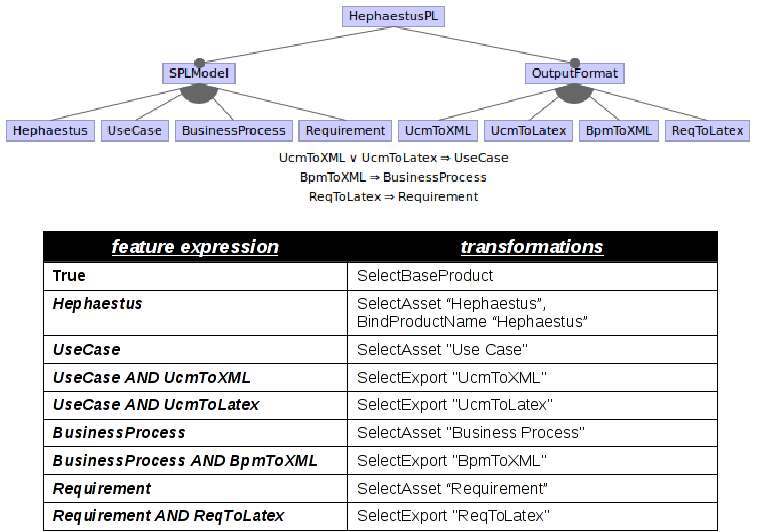
\includegraphics[scale=0.6]{imagens/fm-ck-hpl-req.png}
%\end{center}
%\caption{Hephaestus-PL's FM and CK after introducing \textit{Requirement} asset.}
%\label{fig:fm-ck-hpl-req}
%\end{figure*}

\begin{figure*}[bth]
\begin{center}
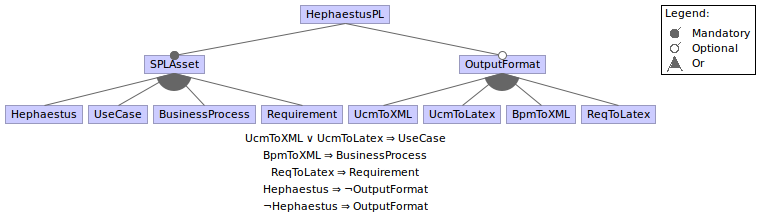
\includegraphics[scale=0.5]{imagens/fm-hpl-ucm-bpm-req.png}
\end{center}
\caption{Hephaestus-PL's FM after introducing \textit{Requirement} asset.}
\label{fig:fm-hpl-ucm-bpm-req}
\end{figure*}

\begin{table}[h]
\begin{center}
\begin{tabular}{||l||l||}
  \hline
  \textbf{Feature Expressions} & \textbf{Transformations}   \\  \hline
  True                         & SelectBaseProduct \\  \hline
  Hephaestus                   & BindProductName "Hephaestus" \\ 
                               & SelectAsset "Hephaestus"   \\
                               & RemoveProductMainFunction \\ \hline
  NOT Hephaestus               & SelectCKParser \\ \hline  
  UseCase                      & SelectAsset "Use Case" \\ \hline
  UseCase AND UcmToXML         & SelectExport "UcmToXML"  \\ \hline
  UseCase AND UcmToLatex       & SelectExport "UcmToLatex" \\ \hline
  BusinessProcess              & SelectAsset "Business Process" \\ \hline
  BusinessProcess AND BpmToXML & SelectExport "BpmToXML" \\ \hline
  Requirement                  & SelectAsset "Requirement" \\ \hline
  Requirement AND ReqToLatex   & SelectExport "ReqToLatex" \\ \hline
\end{tabular}
\caption{Hephaestus-PL's CK after introducing \textit{Requirement} asset.}
\label{tab:ck-hpl-ucm-bpm-req}
\end{center}
\end{table}


Finally, the domain engineer generates a product \hpl{} instance by selecting a product configuration only with the new \textit{Requirement} asset integrated into \hpl{}. She validates if the generated instance contains the correct definitions of the \textit{Requirement} asset into points of variability of the \hpl{} base product and reported the new \hpl{} version to application engineer. Suppose that the validation of the integration of \textit{Requirement} asset into \hpl{} has not been successfully, then it is necessary to return to the assessment of impact in the \hpl{} Kernel's APIs until the validation correct of \hpl{} instance.
 
%The detailed description of the activities of the Hephaestus-PL's reactive process are presented in Appendix B. 

%\subsection{Design Rules for a minimum asset metadata structure}
%\label{sec:designRules}

%\textit{Design Rules} represent a mechanism that would allow reduction of the size of the asset metadata structures in \hpl. Using a inference process into the asset modules, especially the modules that define the data types and the transformations of the asset, it would be possible to get the informations, currently contained in the asset metadata structures, to extend the points of variability of a \hpl{} base product. In this case, we could reduce the size of the asset metadata structures to zero.
%Another intermediate solution that would bring a good reduction of the asset metadata structures would work with two informations, a \textit{acronym} and a \textit{name} of asset, and deriving most of the other informations to the points of variation of \hpl{} with these two variables.

%A atual definicao para a estrutura de meta dados do asset contem 16 fields e esta apresentada na Figure~\ref{fig:metaDataCurrent}. Se analisarmos o preenchimento dessa estrutura para cada um dos assets suportados por Hephaestus-PL, observamos que varios fields dessa estrutura apresentam determinada padronizacao e convencoes no seu preenchimento. Como exemplo, podemos citar o nome do tipo de dados que define as transformacoes dos assets UCM, BPM, Requisitos e Componentes: UseCaseTransformation, BusinessProcessTransformation, RequirementTransformation e ComponentTransformation. Ou seja, todos terminam com a string "Transformation" e comecam com o nome do asset. Poderiamos definir que o nome do tipo de dados algebrico que representa as transformacoes do asset deve ser identificado por \texttt{<assetName>++"Transformation"}. Assim sendo, propomos um conjunto de design rules para o desenvolvimento dos artefatos do asset (tipos abstratos de dados, transformacoes e parser) para minimizar o tamanho da estrutura de meta dados do asset em Hephaestus-PL, otimizando recursos e possibilitando maior automacao na geracao da instancia de Hephaestus com a derivacao automatica de alguns insumos para as operacoes de metaprogramacao, hoje integralmente definidos na estrutura de meta dados do asset (Figure~\ref{fig:exampleMetaDataCurrent}).


%A proposta para uma es%trutura de meta dados minima do asset contem 8 fields (reducao de 50\% do tamanho atual) e esta apresentada na Figure~\ref{fig:proposalMinimumMetaData}. Nesse caso, definimos as seguintes restricoes para permitir a automacao da geracao dos elementos de variacao do asset usados pelas operacoes de metaprogramacao:
%
%\begin{itemize}
%
%\item Os valores definidos para cada field da estrutura de meta dados deve ser unico para aquele field em todos os assets de Hephaestus-PL. Exemplo: não e permitido que o field \texttt{<assetSigla>} seja definido como "XPTO" para o asset A e para o asset B.
%
%\item Implementar nos artefatos do asset as seguintes leis de formacao para a identificacao dos elementos usados na geracao do modulo instancia de Hephaestus:
%
%\begin{itemize}
%
%\item nome do modulo com os tipos abstratos de dados do asset deve ser "Types"
%\item nome do modulo parser do asset deve ser \texttt{<assetModuleParser>}
%\item modulo parser do asset deve estar localizado abaixo do diretorio \texttt{<assetSigla>/Parsers}
%\item nome da funcao parser do asset dentro do modulo do parser (\texttt{<assetModuleParser>}) deve ser \texttt{"parse"++<assetName>++"File"}
%\item nome do modulo que implementa as transformacoes do asset deve ser \texttt{<assetName>}
%\item nome do tipo de dados algebrico que representa o asset deve ser \texttt{<assetName>++"Model"}
%\item nome da funcao que define um produto vazio do asset deve ser \texttt{"empty"++LowerCase<assetSigla>}
%\item nome do tipo de dados algebrico que representa as transformacoes do asset deve ser \texttt{<assetName>++"Transformation"}
%\item nome da funcao que define as transformacoes do asset deve ser \texttt{"transform"++LowerCase<assetSigla>}
%\item nome do parametro que define o asset PL no arquivo de propriedades da entrada de Hephaestus deve ser \texttt{LowerCase<assetName>++"-model"}
%
%\end{itemize}
%
%\end{itemize}
%
%A Figure~\ref{fig:exampleMetaDataMinimum} apresenta um exemplo da estrutura de meta dados minima para o asset UCM.
%
%As regras e definicoes para a automacao da derivacao das informacoes usadas pelas operacoes de metaprogramcao estão sintetizadas na Figure~\ref{fig:metaDataCurrentDerivation} que apresenta a associacao entre os fields da estrutura de meta dados atual e a definicao dos fields a partir da proposta apresentada na Figure~\ref{fig:proposalMinimumMetaData}.


\begin{figure*}[bth]
\begin{center}
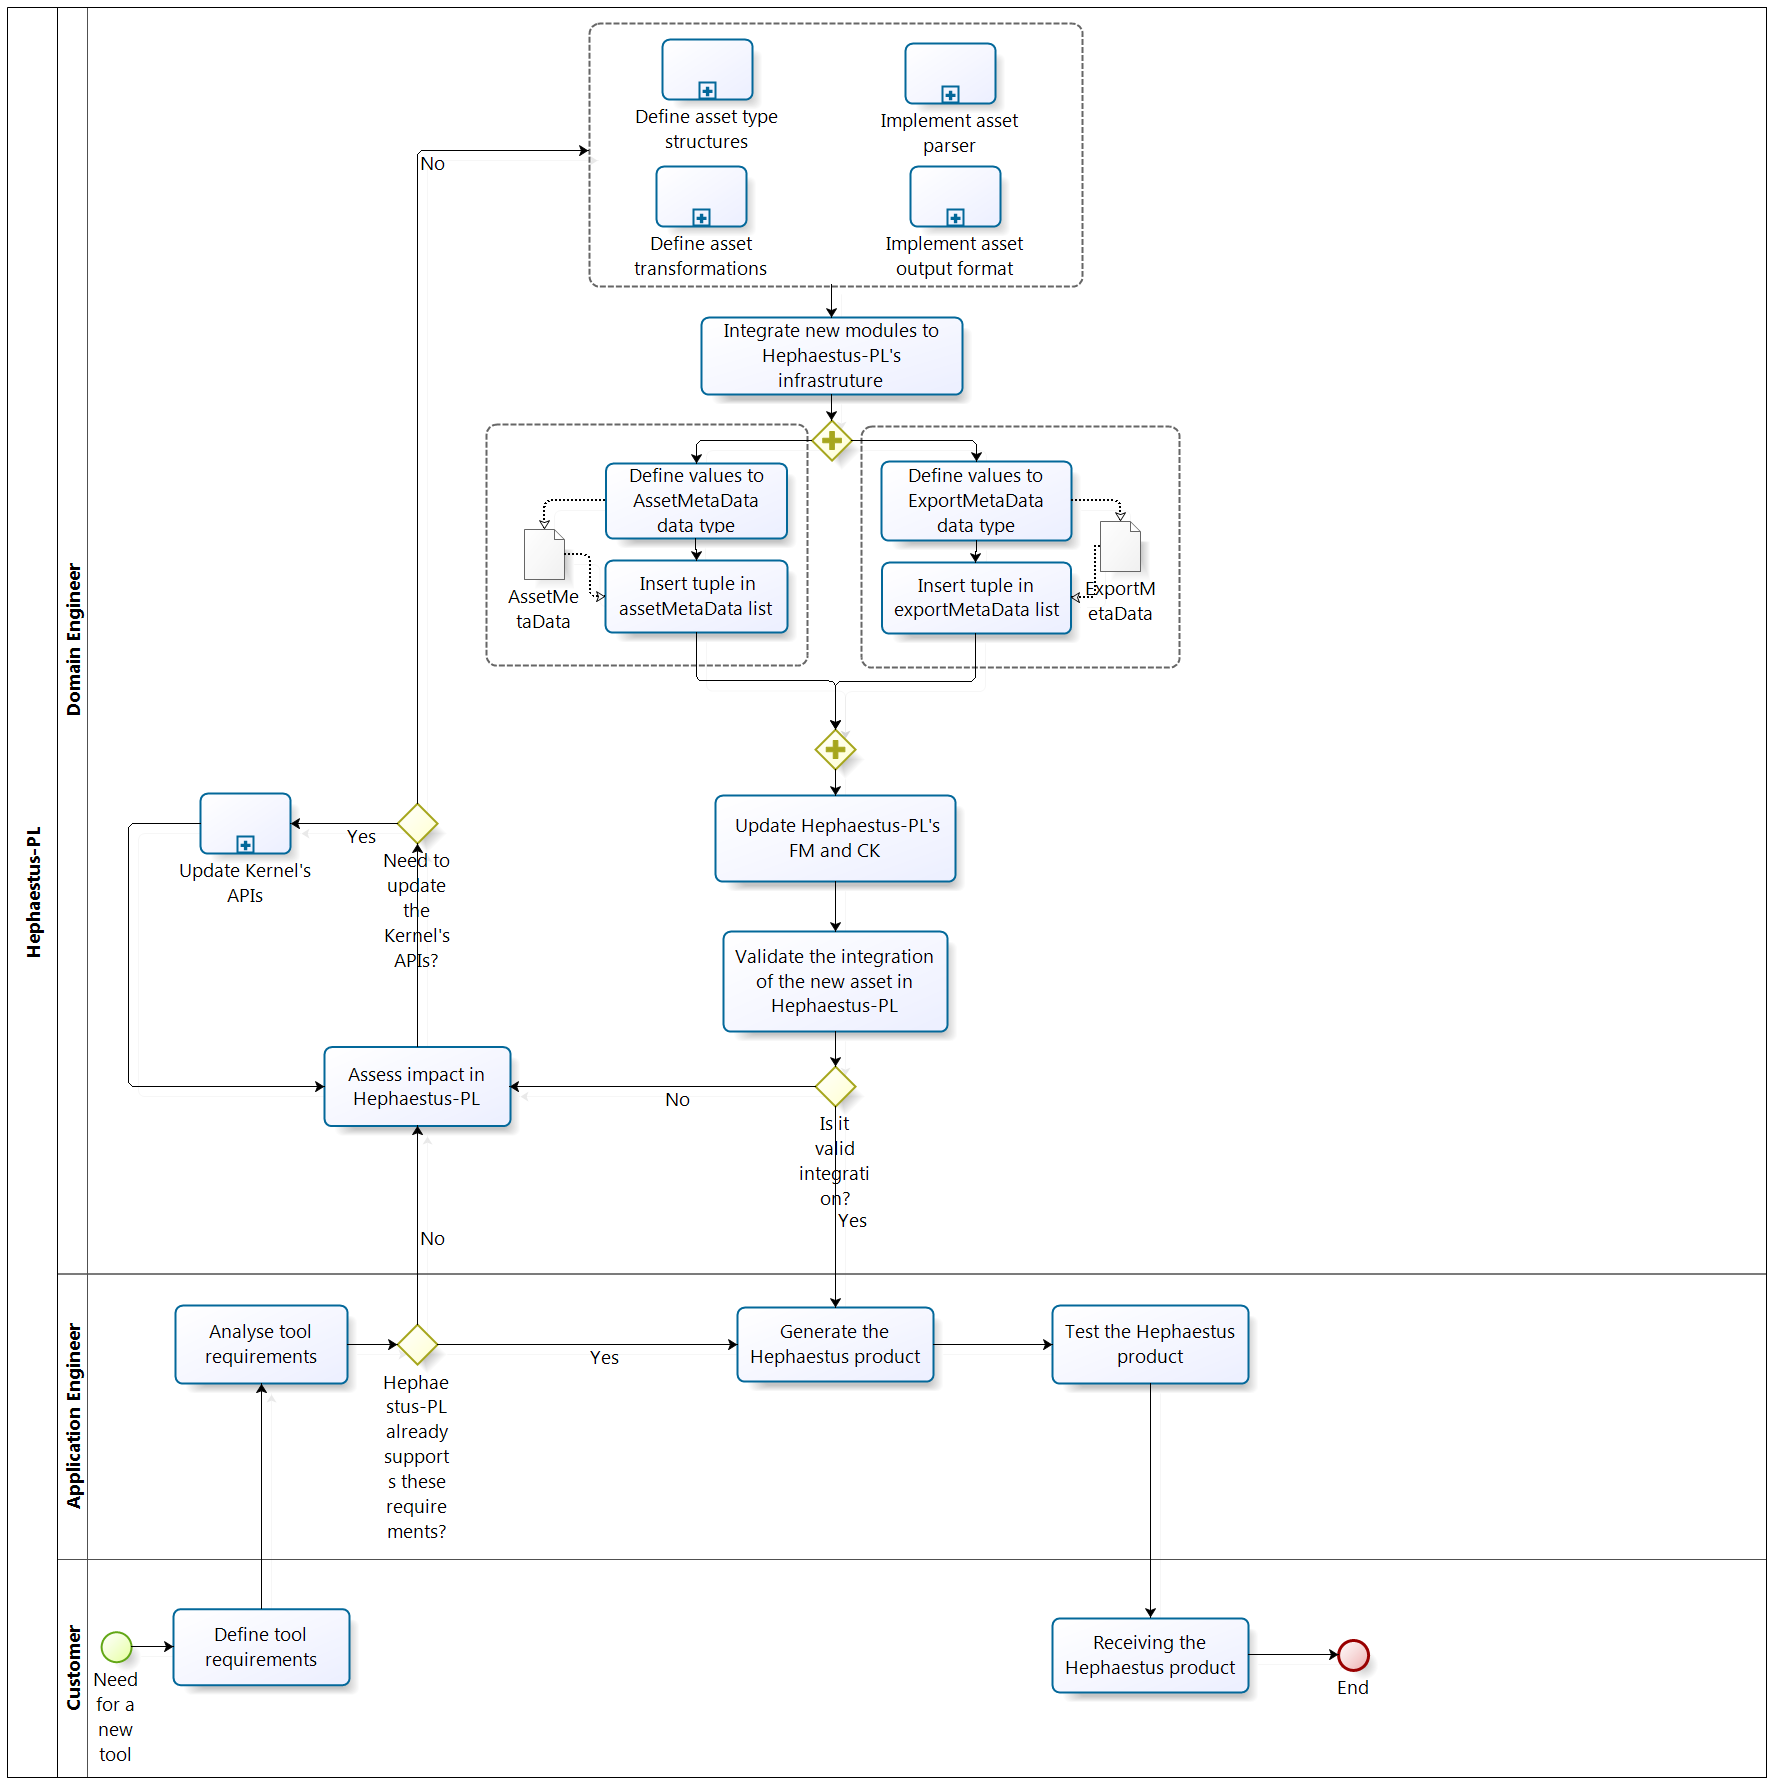
\includegraphics[scale=0.35]{imagens/process.png}
\end{center}
\caption{Reactive Process for introducing new artifacts in \hpl.}
\label{fig:process}
\end{figure*}

%Alem disso, se a variabilidade dos assets nos data types \textit{SPLModel} e \textit{InstanceModel} fosse definida apenas com a adicao de um field que representasse o data type do asset então, poderiamos na geracao de um produto Hephaestus derivar o field e seu tipo a partir dos fields \texttt{<assetSigla>} e \texttt{<assetName>} da estrutura de meta dados minima proposta (ver situacao atual e a proposta na Figure~\ref{fig:proposalAssetSelector}). Atualmente, esse comportamento descrito aqui e observado para os assets UCM, BPM e Requisitos em \hpl. Porem, o asset Componentes não tem esse mesmo comportamento no \textit{SPLModel} e \textit{InstanceModel}, conforme apresentado
%na Section~\ref{sec:implementation}. Assim sendo, precisamos manter os fields  assetSelector' e assetSelector na estrutura de meta dados do asset para atender a extensão desses data types \textit{SPLModel} e \textit{InstanceModel} na geracao da instãncia \hp.
%
%
%
%
%


\section{Results and Discussion}
\label{sec:results-discussion}


%\section{Study Settings} \label{study-settings}

In order to guide the discussion of the results, we apply the Goal Question Metric (GQM) method~\cite{gqm}, so that it helps structuring the context, the object of study, its properties, the goal, and how this latter can be operationalized and answered. In this section we first discuss the goals, questions and metrics of our investigation (Subsection~\ref{sec:gqm}), then evaluate our empirical study  accordingly (Subsection~\ref{sec:assessment}), and finally discuss its limitations (Section~\ref{sec:threats}).

\subsection{Goals, Questions, and Metrics} \label{sec:gqm}

Our goal is to assess the configurability and flexibility of \hpl{} (Sections~\ref{sec:domainDesign} and~\ref{sec:implementation}), regarding the application engineering phase for software product development and within the context of the different artifacts.  Since \hpl{} emerged from a systematic evolution of \hp{}, this later is also assessed as a baseline. According to GQM, Table~\ref{tab:gqm-goal} summarizes the general evaluation goal of our work.

\begin{table}[h]
\begin{center}
\begin{tabular}{||l||l||}
  \hline
  \textbf{Purpose} & assess   \\  \hline
  \textbf{Issue} & the configurability and flexibility of\\  \hline
  \textbf{Object} & \hpl{} and \hp  \\ \hline
  \textbf{Viewpoint} & application engineering perspective  \\ \hline
  \textbf{Context} & different artifacts  \\ \hline
\end{tabular}
\caption{GQM goal of this research.}
\label{tab:gqm-goal}
\end{center}
\end{table}

In Section~\ref{sec:hephaestus}, we characterized the \emph{context}, the \emph{viewpoint}, and part of the \emph{object} of the initial Hephaestus design, which was targeted
to manage variability in use case scenarios, and its evolution to support variability in other assets.
In Sections~\ref{sec:domainDesign} and~\ref{sec:implementation}, we detailed part of the \emph{object}, i.e., \hpl.
This section proceeds with the analysis of \hpl{} and \hp{}, using a qualitative and quantitative evaluation that answers our GQM metrics, thus meeting the \emph{purpose} and \emph{issue} components of the study's goal.

From the study's goal presented in Table~\ref{tab:gqm-goal}, we derive questions that best characterize our study. Moreover,
related to each question, we use one or more quantitative or qualitative metrics to indicate the compliance level of the techniques in relation to
the study goal. Qualitative assessment ``metrics" are also conceived in the GQM method~\cite{gqm}.
In what follows, we present the questions (\textbf{Q}) and the metrics (\textbf{M}) of our GQM model and explain how they trace to the study's goal.

\begin{enumerate}[Q1]
\item \emph{Is the variability mechanism sufficiently expressive?}
\begin{itemize}
\item Metric \textbf{M1.1}: Is there support for open data types?
\item Metric \textbf{M1.2}: Is there support for open functions?
\item Metric \textbf{M1.3}: Is there support for the instantiation of one SPL asset?
\item Metric \textbf{M1.4}: Is there support for the composition of assets without having to instantiate all assets (over features)?
\end{itemize}

\item \emph{Given a fixed number of assets, what is the effort to address a new configuration?}
\begin{itemize}
\item Metric \textbf{M2.1}: Number of modules changed.
\item Metric \textbf{M2.2}: Number of lines of code changed.
\item Metric \textbf{M2.3}: Number of modules created.
\item Metric \textbf{M2.4}: Number of lines of code created.
\item Metric \textbf{M2.5}: Is there automation support?
\item Metric \textbf{M2.6}: What is the analytical complexity of the effort?
\end{itemize}


\item \emph{What is the effort to address a new asset?}
\begin{itemize}
\item Metric \textbf{M3.1}: Number of modules changed.
\item Metric \textbf{M3.2}: Number of code artifacts changed.
\item Metric \textbf{M3.3}: Number of modules created.
\item Metric \textbf{M3.4}: Number of code artifacts created.
\item Metric \textbf{M3.5}: Is there automation support?
\end{itemize}

%@all: should we use a metric like degree of scattering below? also degree of tangling?
\item \emph{Is modular management of asset related variability supported?}
\begin{itemize}
% \item Metric \textbf{M4} (Yes/No): The technique provides support for feature modularization.
\item Metric \textbf{M4.1}: Are the changes related to variability of SPL asset homogeneous or heterogeneous?
\item Metric \textbf{M4.2}: Are the changes related to variability of SPL asset localized or scattered?
\item Metric \textbf{M4.3}: What is the possibility of automation of the changes related to variability of SPL asset?
%\item Metric \textbf{M4.4}: What is the value for the Concern Diffusion over Components (CDC) metric?
%\item Metric \textbf{M4.5}: What is the value for the Concern Diffusion over Operations (CDO) metric?
\end{itemize}
\end{enumerate}


%@Lucineia: please ensure that in  Section 3.1 (Domain Analysis) we make this classification or give elements so that we can say we address such things in the paragraph below.
%           In Section 3.1, after the final bullet list, please add this discussion.  We only slight mention this in Seciton 2.1.
Questions Q1-Q4 represent relevant characteristics of the development of \hpl{} when compared to \hp. Q1 traces to the configurability issue, addressing the required expressiveness of the underlying variability management mechanism. Correspondingly, Metrics M1.1, M1.2, M1.3 and M1.4 investigate whether there is support for the types of variability in Hephaestus-PL, classified as open data types, open functions, single asset instantiation, and assets composition, as explained in Section~\ref{sec:domainAnalysis}.
In particular, metric M1.4 focuses on a current issue of Hephaestus: the need to instantiate more than one SPL asset defined in \texttt{SPLModel} and \texttt{InstanceModel} algebraic types.
Likewise, Q2 also deals with the configurability issue, but addresses it within a predefined scope of assets. Its metrics then address the effort to add a new configuration, from different granularity perspectives (modules and lines of code), automation support, and analytical complexity, the latter being relevant for scalability.
Differently, Q3 traces to the flexibility issue, by considering the necessary evolution effort to address variability in a new asset. This question is refined by metrics from different granularity perspectives (code artifacts represent data types and functions, except modules) and also considering automation support. Finally, Q4 also refers to the flexibility issue and assesses whether modularity in handling asset related variability is supported or not, an important property to the reactive approach for SPL development since it potentially supports the introduction of new features. 
The homogeneity (metric 4.1) refers to the kinds of Haskell syntactic structures (data types, functions, classes) associated with the changes. We consider homogeneous when there is only one type of syntactic structure to change and heterogeneous otherwise. 
The location of the changes (metric 4.2) is assessed on the modules with tangled code of features and can be defined as localized when it involves only one module or scattered otherwise. 
At the end, the metric M4.3 is defined as a result of metric M4.1 and M4.2. Thus, M4.3 can be high when we observe the values homogeneous to M4.1 and located to M4.2 otherwise we define M4.3 as low.



\subsection{Assessment} \label{sec:assessment}

Given the GQM setup from Subsection~\ref{sec:gqm}, we now proceed to evaluating the design and implementation techniques for managing variability (Sections~\ref{sec:domainDesign} and~\ref{sec:implementation}). Table~\ref{tab:assessment-hpl-hp} summarizes the assessment to \hp{} and \hpl{} of the metrics associated to questions defined in the our GQM model.


\begin{table}[h]
\begin{center}
\begin{tabular}{||c|| p{5cm} || p{5cm}||}
  \hline
  \textbf{Metric} & \textbf{Hephaestus} & \textbf{Hephaestus-PL}   \\  \hline  \hline 
  \textbf{M1.1} & No  & Yes \\  \hline
  \textbf{M1.2} & No  & Yes \\  \hline
  \textbf{M1.3} & Yes & Yes \\  \hline
  \textbf{M1.4} & No  & Yes \\  \hline \hline   
  \textbf{M2.1} & 1  & 0 \\  \hline
  \textbf{M2.2} & $9n$  & 0 \\  \hline
  \textbf{M2.3} & 0  & 0 \\  \hline
  \textbf{M2.4} & $8n$  & 0 \\  \hline  
  \textbf{M2.5} & No & Yes \\  \hline  
  \textbf{M2.6} & $O(n)$ & $O(k)$ \\  \hline  \hline 
  \textbf{M3.1} & 5  & 1 \\  \hline
  \textbf{M3.2} & 6  & 4 \\  \hline
  \textbf{M3.3} & 4 & 4 \\  \hline
  \textbf{M3.4} & low, depends of new asset &  low, depends of new asset \\  \hline  
  \textbf{M3.5} & No & No \\  \hline \hline 
  \textbf{M4.1} & heterogeneous  & homogeneous \\  \hline
  \textbf{M4.2} & scattered      & localized \\  \hline
  \textbf{M4.3} & low            & high \\  \hline
%  \textbf{M4.4} & ?              & ? \\  \hline
%  \textbf{M4.5} & ?              & ? \\  \hline  
%  \textbf{M4}   & No (heterogeneous and scattered changes) & Yes (homogeneous and localized changes)  \\  \hline \hline        
\end{tabular}
\caption{Summary of the assessment of the metrics of GQM model}
\label{tab:assessment-hpl-hp}
\end{center}
\end{table}


Regarding Q1, when evaluated in \hpl{}, there is sufficient expressiveness to support all variability types in Hephaestus.
The support for variability in data types and functions (metrics M1.1 and M1.2) is guaranteed by the transformational approach of variability management used in \hpl{}, i.e., using metaprogramming operations 
%with the support of meta data structure containing SPL asset informations we 
to extend the data types and functions.
The support for the composition of assets, i.e., instantiation of a product with one or more assets (metrics M1.3 and M1.4) is guaranteed by the \texttt{build} process of the \hpl's kernel and metaprogramming operations generating a \hpl{} variant that represents an instance of product which combines any assets of the \hpl's Feature Model.
When evaluated in \hp{}, that is a variant manually generated that supports derivation of products using a compositional approach of artifacts and transformations into CK to generate a new product, we observe there is not support for variability management in data types and functions by the introduction of new assets and for the composition of any assets. 
%In the first \hp{} variant the variability management of use case scenarios used MSVCM (Modeling Scenario Variability as Crosscutting Mechanisms) such as aspects' concept. 
Related to M1.4, the generation of \hp{} variant that supports a composition of assets without having to instantiate all assets requires noticiable effort because it is necessary to change several code artifacts (modules, data types and functions). 
This \textit{ad hoc} change in different parts of the code is an error-prone activity and it is not usually done. Alternatively, we could use the concept of \textit{Over Feature} to generate new \hp{} variants because the impact is considered small and limited into \texttt{main} function.

%The support for variability in data types, functions and the composition of assets is guaranteed by operations in the meta-programming module in the process of generating a variant that represents an instance of product which combines any assets of the SPL Feature Model.....

Regarding Q2, when evaluated in \hpl{}, the effort to address a new configuration from a fixed number of assets is constant and small and represents the effort to specify the new product configuration for \hpl{} with the selected assets, whereas the assets of the desired configuration are already integrated into \hpl. Therefore, a measure for the metric M2.6 is constant and close to zero ($\simeq O(k)$). Likewise, the measure for the metrics M2.1, M2.2, M2.3 and M2.4 is zero, i.e., there are not created and modified modules. Regarding the metric M2.5, there is an automation support in \hpl{} to generate new asset configurations based on the \texttt{build} process, \hpl's transformations and operations of metaprogramming which treat the variability in \hpl.

When evaluated in \hp{}, the effort to address a new configuration of assets can be seen in two ways: by using or not the concept of \textit{Over Feature}. 
First, using the concept of \textit{Over Feature} and a \hp{} product that supports a set of assets where the desired configuration is a subset of these assets, the effort is considered small with impact only on the \texttt{Main.hs} module that needs some changes in
the code. Therefore, the measure of the metric 2.1 is one module and the measure of the metric 2.3 is zero module (i.e., no module is created). Lines of code related to selected assets are changed and created in the module \texttt{Main.hs}, i.e., importing the modules of algebraic data types, parser and output format, reading the SPL asset file in the input \hp{} properties file, executing the asset parser, updating the \texttt{createSPL} function after execute the asset parser
%, inserting the definition of empty asset into empty product function for the build process 
and executing the call of the export function of the asset in the output format. This represents about nine changed lines (metric M2.2) and eight created lines (metric M2.4) in \texttt{Main.hs} module. 
%In \texttt{ConfigurationKnowledge/Interpreter.hs} module are introduced about four new lines to the definition of empty asset into empty product function for the \texttt{build} process. 
With respect to the metric M2.5 there is not automation support in \hp{} and analytical complexity of the effort (metric M2.6) using the concept of \textit{Over Feature} in \hp{} is the sum of the number of changed and created lines (metric M2.2 and M2.4) multiplied by the number of assets ($n$) of the desired configuration, i.e., $(M2.2 + M2.4) * n \simeq O(n)$. Therefore, the effort is proportionally linear to the number of assets of the configuration.

Analyzing now the effort to address a new configuration of assets when we did not use \textit{Over Feature} in \hp{}, we observe that the impact is quite high because it is necessary to introduce into the \hp{} variant the code related to selected assets and this requires a good understanding the code and changes in several modules, data types and functions. Moreover, being a manual activity is more error-prone and to check invalid settings is not an easy task to be done manually. Thus, only to use code of the assets of the selected product configuration would be necessary to copy the source code of \hp{} variant to a new directory and remove the non-selected features. Currently \hp{} does not work like this.

Regarding Q3 refers to reactive process, both \hpl{} and \hp{} tools, the effort to address a new asset considers the major and initial effort to generate the elements of the new asset, such as the abstract data types, the transformations, the parser function and the output format function. This effort is the same in both tools and assessing it is outside the scope of this paper. After generation of asset's elements, there is the effort to integrate these elements of new asset into \hpl{} and \hp{}. We evaluate this later effort.
When evaluated in \hpl{}, the number of changed modules and code artifacts (metrics M3.1 and M3.2) is only one changed module (\texttt{MetaData.hs}) and four changed code artifacts. In \texttt{MetaData.hs} module we need to change the \texttt{featuremodel} and \texttt{configurationKnowledge} functions that build the \hpl's FM and CK and to change the \texttt{assetMetaData} and \texttt{exportMetaData} lists that contain the meta data structures that support metaprogramming operations. The number of created modules and code artifacts (metrics M3.3 and M3.4) are four created modules (\texttt{Types.hs} contains the algebraic data types, \texttt{<NewAsset>.hs} contains the transformations that manage asset's variabilities, \texttt{<NewAssetFomartParser>.hs} contains the asset parser function and \texttt{<NewAssetOutputFormat>.hs} contains a asset output format function) where the sum of created code artifacts (data types and functions) varies depending on the asset. 
%Besides, we have up to fifty created lines of code in the \texttt{MetaData.hs} module.
Currently, there is not automation support in \hpl{} to address a new asset (metric M3.5) but it is possible in the future using a minimum set of variables with the automatic or semi-automatic derivation of the asset meta data informations into asset elements since the meta data estructures have a regular structure and the implementation of asset follow some design rules to enable this automatic or semi-automatic derivation. 
% in the future they may suffer simplifications to automate and derive some informations to execution of the metaprogramming operations.
When evaluated in \hp{}, the number of changed modules and code artifacts (metrics M3.1 and M3.2) are five changed modules (\texttt{ConfigurationKnowledge/Types.lhs}, \\ \texttt{ConfigurationKnowledge/Interpreter.hs}, \\ \texttt{Parsers/XML/XmlConfigurationKnowledge.hs}, \\ \texttt{ExportProduct.hs} and \texttt{Main.hs}) and six changed code artifacts that are \texttt{SPLModel} and \texttt{InstanceModel} data types and \texttt{build}, \texttt{xml2Transformation}, \texttt{exportProduct} and \texttt{main} functions.
The number of created modules and code artifacts (metrics M3.3 and M3.4) are also four created modules (\texttt{Transformations/<newAsset>.hs}, \texttt{<newAsset>/Types.hs}, \\ \texttt{<newAsset>/Parsers/<newAssetParser>.hs} and \\  \texttt{<newAsset>/PrettyPrinter/<newAssetOutputFormat>.hs}) and the number of created code artifacts to represent the elements of the new asset (abstract data types, transformations, parser function and output format function) varies depending on the asset.
In both \hpl{} and \hp{} the number of changed and created code artifacts is small because Haskell is a declarative (functional) language.
In \hp{} there is not automation support to address a new asset (metric M3.5) and it is more difficult than \hpl{} to implement some automation because in \hp{} asset code is scattered in five modules and its format is heterogeneous. 
%As consequence, it becomes more difficult to understand, maintenance and reuse of code besides the possibility of evaluating a automation support.

In terms of feature modularization (Q4), we observe that both \hpl{} and \hp{} support modularity in the elements of SPL asset which are defined in independent modules and have their implementation entirely confined to specific modules, like the four modules that define respectively the algebraic data types, transformations, parser and output format of the asset.
However, there is code associated with SPL asset that is scattered and tangled with code from other SPL asset in some modules. Therefore, to assess if the management of SPL asset related variability is modular we define three metrics.
We evaluate the homogeneity (metric M4.1), the location (metric M4.2) and the possibility of automation (metric M4.3) of the changes related to variation points of SPL asset in the \hpl{} and \hp{} objects as qualitative criteria for the Q4 question. 
%In addition, we use two metrics related to concerns (SPL assets) that are already known, Concern Diffusion over Components (CDC) and Concern Diffusion over Operations (CDO). CDC was applied to the modules and CDO was applied to the functions related concerns.
In \hp{} we define the changes to address an SPL asset as heterogeneous, scattered and therefore with lower possibility of automation. They are heterogeneous because they refer to different types of changes such as insertion of fields in data types, defining new class instances, defining new functions and introducing new sentences in functions. The changes are scattered because they occur in five different \hp{} modules (as presented in \hp{}'s metric M3.1) and 
%\hp{} does not have modular support for the variability management of SPL asset. 
the \hp{} modules that address variability of SPL asset need to be updated manually and it is a error-prone activity (i.e., changes are heterogeneous, scattered in various modules and tangled with other SPL assets). 
%The modularity of transformations in CK and of \textit{build} process respond only to product line's variability management supported in \hp{}.
On the other hand, in \hpl{} the changes to address new assets are classified as homogeneous and localized since they only refer the definition of SPL asset meta data informations in a single \texttt{MetaData.hs} module. Thus, in \hpl{} there is more possibility of automation from a process of inference into the SPL asset modules implemented according to design rules previously defined.
We had a initial greater effort in the development of \hpl{} with the participation of a Haskell expert creating an infrastructure that contributes to a reduced effort to address the changes related to new assets when compared to the effort for the same purpose observed in \hp.

Furthermore, in \hpl{} some degree of modularity was obtained by the mapping of \hpl's product configurations to metaprogramming transformations where the \hpl's variability related to the assets' configuration is handled dynamically and automatically in the generation of a \hpl{} variant. This is allowed by the transformational process of generating products in \hpl{} with the support of the metaprogramming operations that meet the needs of managing the variability of assets in the artifacts (open data types and open functions) of the base module of \hpl.

%In addition, in \hpl{} the features represented by assets have their implementation entirely confined to specific modules, like the four modules that define respectively the algebraic data types, transformations, parser and output format of the asset.

%In addition to these results, we make some considerations on important issues like type safety and...

%Finally, regarding type safety, the generated instances are well-formed. A formal reasoning for type safety of the generation is beyond of the scope of this work. Instead, in the following, we present an analytical argument on type safety of the generated variants of \hpl. The \textit{build} performed by the kernel operates on a base product, which itself is well-formed. The metaprogramming transformations performed by the kernel are any of the following: add field, add constructor, add sentences in function, add import clause. Each of these takes a well formed program as input and generates a well-formed program as output...

\subsection{Threats to Validity} \label{sec:threats}

The threats to validity of our study can be addressed as follows:

\begin{itemize}

\item \emph{Construct validity} concerns establishing correct operational measures for the concepts being studied. The main constructs in our study are the concepts of ``configurability" and ``flexibility". Regarding the first, we defined metrics considering the underlying variability and effort of adding a configuration. As for the second construct, we defined metrics considering the evolution effort to address a new asset as well as key internal characteristic such as modularity.

\item \emph{Internal validity} concerns establishing a causal relationship, whereby certain conditions are shown to lead to other conditions. The design decisions behind the architecture definition trace to solving variability issues demanded by enhanced configurability support. The proposed reactive process was conceived to address the flexibility issue.

\item \emph{External validity} concerns establishing the domain to which a study's findings can be generalized. Although our study focuses on a single tool,  we believe that its design and supporting reactive process could be used to improve configurability and flexibility in other SPL product derivation tools.

\item \emph{Reliability} concerns demonstrating that the operations of a study can be repeated with the same results. Given the design, implementation, and reactive process descriptions, we expect that replications of our study should offer results similar to ours.

\end{itemize}





\section{Related Work}
\label{related-work}

%@vra: to be refined and extended

Previous work discusses the need to address SPL tool development as SPL development itself~\citep{grunbacher:2008}. Nevertheless, detailed guidelines on domain and application engineering were not explored.

As discussed in Section~\ref{sec:domainAnalysis}, a key requirement of \hpl{} is to support or-configurability of product artifacts, which has not been explicitly addressed elsewhere.

In \citep{batory-ahead-bootstrap} was bootstrapped AHEAD from AHEAD. This is similar to our work, but they do not focus on addressing different artifacts and no explicit support for or-feature is provided. Furthermore, the programming language and paradigm is different from ours.

Transkell~\citep{marcos:2010} is a domain specific language (DSL) developed to extract and modularize the variabilities of Hephaestus tool and makes it a product line. It is a technique of transformation approach similar to our work.
%Thus, it offers flexibility to extend the tool to new domains. 
The Hephaestus’s feature model represents the transformations of Hephaestus and the syntax and semantics of the Transkell language were implemented in the environment Stratego/XT~\citep{visser:2003}. In our work, we focus on assets variabilities that represent the different domain artifacts of \hp{} and we present the details of \hpl{} developed as a product line. 

The \textit{DOPLER (Decision-Oriented Product Line Engineering for effective Reuse)} approach~\citep{DBLP:journals/ase/DhunganaGR11} represents a tool suite to SPL tool development as SPL development itself~\citep{grunbacher:2008}. It comprises \textit{DoplerVML}, a variability modeling language to define product lines based decision models with emphasis on the derivation of products.
\textit{DOPLER} was initially developed to support the domain of industrial automation (Siemens VAI), but the proposal to be extensible and customizable to different contexts to meet the needs of different users and organizations.
However, the approach \textit{DOPLER}  does not support configurability of any combination of assets as we propose in the solution of our work.

Some other comparative studies with product derivation tools were conducted ~\citep{DBLP:conf/gpce/TorresKSBTBCLBM10, uiraWBDDM:2010}. 
~\citep{DBLP:conf/gpce/TorresKSBTBCLBM10} has analyzed six modern product derivation tools (Captor, CIDE, GenArch, Hephaestus, pure::variants e XVCL) in the context of evolution scenarios of a software product line. The study analyzed the modularity, complexity and stability of product derivation artifacts along  evolution of a mobile product line. The evaluation showed that  modularity and  stability requirements in software product lines are favorable to the flexibility of the tool.
In ~\citep{uiraWBDDM:2010} the flexibility and extensibility of product line development tools that support product derivation based on DDM and AOSD approaches were evaluated to support the addition of new features.



\section{Conclusion}
\label{conclusion}

Hephaestus-PL is a product line resulting from evolution of the Hephaestus tool. 
Hephaestus~\cite{rbonifacio:sbcars2009} was initially designed to support application engineering and variability management in a product line of use case scenarios.
%To manage the variability in use case scenarios, Hephaestus uses a compositional approach, in particular, aspect-orientation, that combines four input artifacts of the product line (SPL Model, Feature Model, Product Configuration and Configuration Knowledge) to the derivation of product instances.
Over time, Hephaestus evolved to manage variability in other assets such as requirements, source code, and business processes. However, this tool was not designed with flexibility and configurability in mind to allow its customization to address variability in a new specific asset nor in any desired combination of assets.

To address this shortcoming, Hephaestus-PL was developed. 
%It is a software product line that was extracted from different versions of Hephaestus, each version being a tool addressing variability in a number of artifacts.
Hephaestus-PL increases the configurability of Hephaestus by allowing the derivation of instance tools managing variability in any combination of artifacts; additionally, its flexibility allows for further systematic extension to add new assets and their combination. 
%Since Hephaestus-PL was bootstrapped from such independent versions of Hephaestus, \hpl{}'s CK, as well as \hp{}'s CK, represents a mapping of feature expressions to transformations.
%Hephaestus-PL implements six high-level transformations to generate an instance of Hephaestus, namely SelectBaseProduct, SelectAsset, SelectExport, BindProductName, RemoveProductMainFunction and SelectCKParser. 
%These transformations of Hephaestus-PL’s CK are built from a combination of set of meta-programming operations that when executed perform modifications in the product Hephaestus instance being generated.
Once Hephaestus-PL was bootstrapped, we defined a reactive approach to increase its configurability and to reach the goal of enabling the generation of different instances of Hephaestus.

%--talk about assessment
An assessment reveals that \hpl{} has improved configurability and flexibility when compared to previous evolution of \hp.
The proposed \hpl{}'s architecture and the approach of variability management used in \hpl{} address configurability and flexibility in the development of SPL derivation tools. Thus, we using a transformational approach with metaprogramming operations to extend the variation points of the base product of \hpl{} instance. 

In \hpl{} some degree of modularity was obtained by the mapping of \hpl's product configurations to metaprogramming transformations where the \hpl's variability related to the assets' configuration is handled dynamically and automatically in the generation of a \hpl{} variant. This is allowed by the transformational process of generating products in \hpl{} with the support of the metaprogramming operations that meet the needs of managing the variability of assets in the artifacts (open data types and open functions) of the base module of \hpl.
Besides, the reactive process defined in \hpl{} to introduce support for managing variabilities in new assets and it contributes to the flexibility of \hpl{}. 

%--restrictions (limitations) about our work
Although our study focuses on a single tool, we believe that its design and supporting reactive process could be used to improve configurability and flexibility in other SPL product derivation tools.
Nevertheless, further empirical work is necessary to address the external validity threat. 
We also plan to conduct further empirical studies assessing Hephaestus-PL's evolution to handle variability in diferent kind of artifacts.

%--future works
As future work, we propose the definition of \textit{Design Rules} that represent a mechanism that would allow reduction of the size of the asset metadata structures in \hpl. Using an inference process into the asset modules, especially the modules that define the data types and the transformations of the asset, it would be possible to exctract information, currently contained in the asset metadata structures, to extend the variability points of a \hpl{} base product. In this case, we could reduce the size of the asset metadata structures.
Another intermediate solution that would bring a good reduction of the asset metadata structures would work with two pieces of information, a \textit{acronym} and a \textit{name} of asset, and deriving most of the other pieces to extend the variation points of \hpl{}.



%\section{Hephaestus}
%\label{sec:hephaestus}









%% The Appendices part is started with the command \appendix;
%% appendix sections are then done as normal sections
%%\appendix

%\section{Appendix A : Metadata Structures}
\label{sec:appendixA}

The \texttt{AssetMetaData} data type contains the following fields outlined below:

\begin{itemize}
 
\item \texttt{assetModuleType}: contains the module name where are the definitions of abstract data types of the \textit{<newAsset>}. Format: \texttt{<NewAssetDirectory>.Types}

\item \texttt{assetModuleParser}: contains the module name where is implemented the \textit{parser} function of the \texttt{<newAsset>}. Format: \texttt{<NewAssetDirectory>.Parsers.<NewAssetFomartParser>}

\item \texttt{assetModuleType'}: contains the module name where are the definitions of \texttt{SPLModel}, \texttt{InstanceModel}, \texttt{TransformationModel} and \texttt{ConfigurationKnowledge} data types. This module must be imported into generated Hephaestus instance module. Format: \texttt{TestTypes}

\item \texttt{assetModule}: is the module name containing the definitions the \texttt{empty<NewAsset>} and \texttt{transform<NewAsset>} functions. This module must be located below \texttt{HplAssets} directory. Format: \texttt{<NewAsset>}

\item \texttt{assetModel}: is the data type which defines the \texttt{<newAsset>} located in \texttt{Types.hs} module in the \texttt{HplAssets/<NewAssetDirectory>} directory. This data type is used to extend \texttt{SPLModel} and \texttt{InstanceModel} data types in Hephaestus empty instance. Format: \texttt{<NewAsset>Model}

\item \texttt{assetSelector}: is a list of tuples containing the field's name and type to extend the \texttt{InstanceModel} data type to \textit{<newAsset>}. Format: \texttt{[(<nameField>,<typeField>),...]}

\item \texttt{assetSelector'}: is a list of tuples containing the field's name and type to extend the \texttt{SPLModel} data type to \textit{<newAsset>}. Format: \texttt{[(<nameField>,<typeField>),...]}

\item \texttt{assetEmpty}: function name which defines the empty product of the \texttt{<NewAsset>}. Format: \texttt{empty<newAsset>}

\item \texttt{assetXType}: data type's name which defines the constructors of the \texttt{<NewAsset>} transformations. Format: \texttt{<NewAsset>Transformation}

\item \texttt{assetXFun}: function name which defines the implementation of the \texttt{<NewAsset>} transformation functions, located in the \texttt{<newAsset>} module in \texttt{HplAssets} directory. Format: \texttt{transform<newAsset>}

\item \texttt{assetVarProperty}: variable name used to introduce the \texttt{findPropertyValue} instruction into \texttt{main} function of Hephaestus instance to reading the file name which contains the artifacts of \texttt{<NewAsset>} product line. Format: \texttt{<anyString>}

\item \texttt{assetNameProperty}:









\end{itemize}

%% \section{}
%% \label{}

%% References
%%
%% Following citation commands can be used in the body text:
%% Usage of \cite is as follows:
%%   \cite{key}         ==>>  [#]
%%   \cite[chap. 2]{key} ==>> [#, chap. 2]
%%





%% References with bibTeX database:

\bibliographystyle{elsarticle-num}
\bibliography{references}

%% Authors are advised to submit their bibtex database files. They are
%% requested to list a bibtex style file in the manuscript if they do
%% not want to use elsarticle-num.bst.

%% References without bibTeX database:

% \begin{thebibliography}{00}

%% \bibitem must have the following form:
%%   \bibitem{key}...
%%

% \bibitem{}

% \end{thebibliography}


\end{document}

%%
%% End of file `elsarticle-template-num.tex'.
